\documentclass[defaultstyle,10pt,master,Helvetica]{thesis}
%% Enable Latin characters
\usepackage[utf8]{inputenc}
%% Better equations
\usepackage{amsmath, amsthm, amssymb, amsfonts}
%% Used for abreviations??
\usepackage{nomencl}
\renewcommand{\nomname}{List of Abbreviations}
\makenomenclature
%% Advanced tables
\usepackage{multirow}
\usepackage{colortbl}
\usepackage{tabularx}                 
\newcommand{\specialcell}[2][c]{%
  \begin{tabular}[#1]{@{}c@{}}#2\end{tabular}}

%% Better figures
\usepackage{graphics}
\usepackage{epsfig}
\usepackage[hang,small,bf]{subfigure}

%% The two packages are not compatible, and you should use one of the two. Notice however that the
\usepackage[square,numbers,sort&compress]{natbib}

%% Acronyms
\usepackage[printonlyused]{acronym}
\usepackage[acronym]{glossaries}

%% Pseudo-code algorithms
\usepackage{setspace}
\usepackage[ruled,vlined]{algorithm2e}

%% Increase algorithms line spacing
\usepackage{etoolbox}
\AtBeginEnvironment{algorithm}{\setstretch{1.35}}

%% Display JSON 
%\usepackage{bera}% optional: just to have a nice mono-spaced font
\usepackage{listings}
\usepackage{xcolor}

\colorlet{punct}{red!60!black}
\definecolor{background}{HTML}{EEEEEE}
\definecolor{delim}{RGB}{20,105,176}
\colorlet{numb}{magenta!60!black}

\lstdefinelanguage{json}{
    basicstyle=\normalfont\ttfamily,
    numbers=left,
    numberstyle=\scriptsize,
    stepnumber=1,
    numbersep=8pt,
    showstringspaces=false,
    breaklines=true,
    frame=lines,
    backgroundcolor=\color{background},
    literate=
     *{0}{{{\color{numb}0}}}{1}
      {1}{{{\color{numb}1}}}{1}
      {2}{{{\color{numb}2}}}{1}
      {3}{{{\color{numb}3}}}{1}
      {4}{{{\color{numb}4}}}{1}
      {5}{{{\color{numb}5}}}{1}
      {6}{{{\color{numb}6}}}{1}
      {7}{{{\color{numb}7}}}{1}
      {8}{{{\color{numb}8}}}{1}
      {9}{{{\color{numb}9}}}{1}
      {:}{{{\color{punct}{:}}}}{1}
      {,}{{{\color{punct}{,}}}}{1}
      {\{}{{{\color{delim}{\{}}}}{1}
      {\}}{{{\color{delim}{\}}}}}{1}
      {[}{{{\color{delim}{[}}}}{1}
      {]}{{{\color{delim}{]}}}}{1},
}

%% Set links for references and citations in document
\usepackage{hyperref}
\hypersetup{ %a4paper=true,
             colorlinks=false,
             citecolor=red,
             breaklinks=true,
             bookmarks=true,
             bookmarksnumbered=true,
             bookmarksopen=true,
             pdftitle={HOMOPHILIC SELF ORGANIZING FEATURE MAPS: FINDING TOPICS ON SOCIALY CONNECTED DATA, USING SOCIAL NETWORK RELATIONS},
             pdfauthor={Bernardo Simões},
             pdfsubject={Thesis - Master Degree},                  
             pdfcreator={Vim - Bernardo Simões},
             pdfkeywords={thesis, topic detection, twitter, self-organizing maps, classification, clustering}
}

\usepackage{booktabs}
%% Set paragraph counter to alphanumeric mode
\renewcommand{\theparagraph}{\Alph{paragraph}~--}

%% Brian stuff, not sure what
\usepackage{float}
\floatstyle{ruled}
\newfloat{formulation}{thp}{lop}
\floatname{formulation}{Formulation}
\usepackage{enumitem}
\setdescription{style=multiline}

%% Page formatting
\hoffset 0in
\voffset 0in
\oddsidemargin 0.71cm
\evensidemargin 0.04cm
\marginparsep 0in
\topmargin -0.25cm
\textwidth 15cm
\textheight 23.5cm

\usepackage{fancyhdr}
\pagestyle{fancy}
\renewcommand{\chaptermark}[1]{\markboth{\thechapter.\ #1}{}}
\renewcommand{\sectionmark}[1]{\markright{\thesection\ #1}}
\fancyhf{} \fancyhead[LE]{\bfseries\nouppercase{\leftmark}}
\fancyhead[RO]{\bfseries\nouppercase{\rightmark}}
\fancyfoot[LE,RO]{\bfseries\thepage}
\renewcommand{\headrulewidth}{0.5pt}
\renewcommand{\footrulewidth}{0.5pt}
\addtolength{\headheight}{2pt} % make space for the rule
\fancypagestyle{plain}{%
   \fancyhead{} % get rid of headers
   \renewcommand{\headrulewidth}{0pt} % and the line
   \renewcommand{\footrulewidth}{0pt}
}
\fancypagestyle{blank}{%
   \fancyhf{} % get rid of headers and footers
   \renewcommand{\headrulewidth}{0pt} % and the line
   \renewcommand{\footrulewidth}{0pt}
}
\fancypagestyle{abstract}{%
   \fancyhead{}
   \renewcommand{\headrulewidth}{0pt}
   \renewcommand{\footrulewidth}{0.5pt}
}
\fancypagestyle{document}{%
	\fancyhf{} \fancyhead[LE]{\bfseries\nouppercase{\leftmark}}
	\fancyhead[RO]{\bfseries\nouppercase{\rightmark}}
	\fancyfoot[LE,RO]{\bfseries\thepage}
	\renewcommand{\headrulewidth}{0.5pt}
	\renewcommand{\footrulewidth}{0.5pt}
	\addtolength{\headheight}{2pt} % make space for the rule
}
\setcounter{secnumdepth} {5}
\setcounter{tocdepth} {5}
\renewcommand{\thesubsubsection}{\thesubsection.\Alph{subsubsection}}

\renewcommand{\subfigtopskip}{0.3 cm}
\renewcommand{\subfigbottomskip}{0.2 cm}
\renewcommand{\subfigcapskip}{0.3 cm}
\renewcommand{\subfigcapmargin}{0.2 cm}


\begin{document}
\pdfbookmark[0]{Titlepage}{Title}
% IST requires the title page to be written in Portuguese
% IST requires the logo to measure 2cm
\univlogo{3cm}{2cm}{images/IST_A_CMYK_POS.eps}

% OPTIONAL: the thesis logo image
%\thesislogo{2.5cm}{6cm}{images/thesis_logo.eps}

\title{HOMOPHILIC SELF ORGANIZING FEATURE MAPS: FINDING TOPICS ON SOCIALY CONNECTED DATA, USING SOCIAL NETWORK RELATIONS}

\author{Bernardo Simões}
\degree{Engenharia de Redes de Comunicações}
% \otherdegree{Mestre}

\supervisor{Prof. Pável Pereira Calado}
% \othersupervisor{Doutor full name of co-advisor}

\date{Outubro de 2014}

% Only true if thesis was accepted by the jury
\finalthesis{false}

\presidentofjury{Prof. Paulo Jorge Pires Ferreira}
\vogalone{ Prof. Alexandre P. Francisco}
%\vogaltwo{Doutor whatever full name 3}
% \vogalthree{Doutor whatever full name 4}
% \vogalfour{Doutor whatever full name 5}

\maketitle
\clearpage

% On double sided pages. Second page should be white.
% IST requires the cover to appear twice.
\thispagestyle{empty}
\cleardoublepage

\setcounter{page}{1} \pagenumbering{roman}

\baselineskip 18pt % line spacing: -12pt for single spacing
                   %               -18pt for 1 1/2 spacing
                   %               -24pt for double spacing
 
\pdfbookmark{Acknowledgments}{Acknowledgments}
\begin{acknowledgments}
  First of all, I need to thank Professor Pável for introducing me to the world of Machine Learning, without his teachings during the course of web analysis and information extraction, and full support during the development of this thesis. 
  Sofia Martins, for all the support when things got rugher and for proofreading this thesis more times than its humanly bearable.
  To my parents and family, whom dedicated the last 25 years into making me an educated person, and for always worring with my success.
  I need to thank all my friends and coleges from Instituto Superior Técnico, in special to Afonso Oliveira whom was more than a friend, but an actual mentor. Guilherme Vale, Mario Nzualo, Fábio Domingos, João Vasques, João Andrade, David Dias, Rui Costa, Artur Balanuta and probably many more, for all the working hours we have spent together, I couldn't have finished my course without you.
  Finally, to everybody that makes Taguspark Campus probably on the best places to work in the world. It was an awesome journey.
\end{acknowledgments}
 

\pdfbookmark{Abstract}{Abstract}

\begin{abstract}
With the evolution of social media platforms, the amount of unlabeled information has gone skyrocketing. The process of labeling this kind of information is evermore complex. Typical approaches used on the WEB for Topic Detection and Tracking cannot be directly applied due to the small amount of text produced per tweet, orthographic errors, abbreviations and so on.

In this thesis, we propose and analyze a new form of topic detection and tracking on social networks. By leveraging the social relations between authors of the gathered content, and apply them to the clustering process.

In order to achieve this, we proposed some modifications to the artificial neural network  and clustering algorithm --- Self Organizing Maps. 
\end{abstract}

\begin{keywords}
topic detection, twitter, self-organizing maps, classification, clustering
\end{keywords}
\clearpage
\thispagestyle{empty}
\cleardoublepage

\pdfbookmark{Resumo}{Resumo}
\begin{resumo}
 Com a evolução das plataformas sociais, ocorreu um aumento na quantidade de informação não categorizada. No entanto, o processo de categorização deste tipo de informação é bastante complexo, uma vez que os métodos mais comuns de Detecção e Rastreamento de Tópicos na WEB não são directamente aplicáveis em dados criados nas redes sociais. Isto porque o texto produzido por cada tweet é demasiado pequeno, tem muitos erros ortográficos e abreviações, etc.

Nesta tese é proposta e analizada uma nova forma de detecção e rastreamento de tópicos em redes sociais, onde as relações sociais entre os autores do conteúdo foram tidas em conta no processo de clustering.

Para atingir este objectivo, propuseram-se algumas modificações aos Mapas de Kohonen --- um algoritmo de clustering e rede neuronal artificial.
\end{resumo}

\begin{palavraschave}
  detecção de tópicos, twitter, mapas auto organizados, classificação, agrupamento
\end{palavraschave}

\clearpage
\thispagestyle{empty}
\cleardoublepage

% Required for the fancy chapters
\dominitoc
\dominilof
\dominilot
 

%%%%%%%%%%%%%%%%%%%%%%%%%%%%%%%%%%%%%%%%%%%%%%%%%%%%%%%%%%%%%%%%%%%%%%
% List of contents
%\renewcommand{\baselinestretch}{1}
\pdfbookmark[0]{Index}{index}
\pdfbookmark[1]{Contents}{toc}
\tableofcontents
% \contentsline{chapter}{References}{\pageref{bib}}
\cleardoublepage
%\renewcommand{\baselinestretch}{1.5}

%%%%%%%%%%%%%%%%%%%%%%%%%%%%%%%%%%%%%%%%%%%%%%%%%%%%%%%%%%%%%%%%%%%%%%
% List of figures
\pdfbookmark[1]{List of Figures}{lof}
\listoffigures
\cleardoublepage

%%%%%%%%%%%%%%%%%%%%%%%%%%%%%%%%%%%%%%%%%%%%%%%%%%%%%%%%%%%%%%%%%%%%%%
% List of tables
\pdfbookmark[1]{List of Tables}{lot}
\listoftables
\cleardoublepage

% %%%%%%%%%%%%%%%%%%%%%%%%%%%%%%%%%%%%%%%%%%%%%%%%%%%%%%%%%%%%%%%%%%%%%%
% % List of algorithms
% Requires packages algorithmic, algorithm
% \pdfbookmark[1]{List of Algorithms}{loa}
% \listofalgorithms
% \cleardoublepage

% %%%%%%%%%%%%%%%%%%%%%%%%%%%%%%%%%%%%%%%%%%%%%%%%%%%%%%%%%%%%%%%%%%%%%%
% % List of acronyms
\makeglossaries
\pdfbookmark[1]{List of Acronyms}{loac}
\markboth{List of Acronyms}{List of Acronyms}
\chapter*{List of Acronyms}
% This is the ACRONYMS Definition
\begin{acronym}[TDMA]
	\acro{SOM}{Self-Organizing Maps}
	\acro{NLP}{Natural Language Processing}
	\acro{U-Matrix}{Unified Distance Matrix}
	\acro{TF-IDF}{Term Frequency–Inverse Document Frequency}
	\acro{BMU}{Best Matching Unit}
	\acro{LDA}{Latent Dirichlet Allocation}
	\acro{TDT}{Topic Detection and Tracking}
	\acro{VSM}{Vector Space Model}
	\acro{IR}{Information Retrieval}
	\acro{ML}{Machine Learning}
	\acro{ANN}{Artificial Neural Network}
	\acro{MDS}{Multi Dimensional Scalling}
	\acro{PCA}{Principle Component Analysis}
	\acro{URL}{Uniform Resource Locator}
	\acro{JSON}{JavaScript Object Notation}
	\acro{CSV}{Comma Separated Values}
	\acrodefplural{SOM}[SOMs]{Self Organizing Maps}
	\acrodefplural{ANN}[ANNs]{Artificial Neural Networks}
\end{acronym}

\cleardoublepage

% Change pagination from Roman to Arabic.
\setcounter{page}{1} \pagenumbering{arabic}
\baselineskip 18pt
 


\fancychapter{Introduction}
With the evolution of social network websites like Facebook and Twitter, the amount of pertinent content about a specif issue is increasing dramatically, which calls for new ways to make sense and catalog this data.
The usage of social networks for branding quality and on-line marketing is specially compelling since 19\% of all tweets ~\cite{Jansen2009} and 32\% of blog posts~\cite{Melville2009} are about brands or products. Nevertheless, finding topic sensitive information on social networks is extremely complicated due to the fact that documents have very little content, slang vocabulary, orthographic mistakes and abbreviations. \citet{Asur2010} successfully predicted box-office revenues by monitoring the rate of creation of new topics based on debuting movies. Their work outperformed some traditional market-based predictors.

Thus, academic and enterprise worlds started looking at \ac{ML} for new ways to achieve revenue or simply explore and discover patterns in data. 
As a consequence, the \ac{ML} course at Standford is the one with more students enrolling in the year of 2014~\footnote{http://www.forbes.com/sites/anthonykosner/2013/12/29/why-is-machine-learning-cs-229-the-most-popular-course-at-stanford/} with more than 760 students enrolled.

Using unsupervised \ac{ML}, \citet{Le2011} was able to achieved 81.7\% accuracy in detecting human faces, 76.7\% accuracy when identifying human body parts and 74.8\% accuracy when identifying cats. He used a 9-layered locally connected sparse auto-encoder with pooling and local contrast normalization on a large dataset of images (the model has 1 billion connections, the dataset has 10 million 200x200 pixel images downloaded from the Internet). This dataset was trained using model parallelism and asynchronous SGD on a cluster with 1,000 machines (16,000 cores) during three days. Even though the amount of computing power used in this project was of several order of magnitude, it is remarkable how an unsupervised algorithm could achieve such results.

Even though a lot of solutions have arisen in order to automate real time searches, topic categorization and many other data intensive tasks are still done manually. Twitter still uses humans to deliver ads to trending queries, states Edwin Chen's Data Scientist responsible for ads quality at Twitter. On his blog post \footnote{http://blog.echen.me/2013/01/08/improving-twitter-search-with-real-time-human-computation/}, Edwin Chen describes the process of delivering real time adds to trending queries at Twitter. The main problems that arise in the Twitter platform in order to identify rising topics are:
\begin{itemize}
  \item The queries people perform have never before been seen, so it is impossible to know beforehand what they mean.
  \item Since the spikes in search queries are short-lived, there's only a short window of opportunity to learn what they mean.
\end{itemize}
This means that when an event happens, people immediately come to Twitter in order to know what is happening in a determined place. Twitter solves this issue by monitoring which queries are currently popular in real time, using a Storm topology~\footnote{http://storm-project.net/}. After the queries are identified, they are sent to a Thrift API~\footnote{http://thrift.apache.org/} that dispatches the query to Amazon's Mechanical Turk service~\footnote{https://www.mturk.com/mturk/} where real people will be asked a variety of questions about the query.

Social Media Analytics is another raising topic that draws from Social Network Analysis~\cite{knoke2008social}, \ac{ML}, Data Mining~\cite{witten2005data}, \ac{IR}~\cite{salton1983introduction}, and \ac{NLP}. As stated~\citet{Melville2009}, 32\% of the 200 million active bloggers write about opinions on products and brands, while 71\% of 625 million Internet users read blogs and 78\% of respondents put their trust in the opinion of other consumers. In comparison, traditional advertising is only trusted by 57\% of consumers.
This kind of data drives companies to Social Media Analytics as a way to know what people are saying on the web about their companies and products. This new worry has brought to life a lot of new startups like Sumal\footnote{https://sumall.com/} or ThoughtBuzz\footnote{http://www.thoughtbuzz.net/}, but also solutions from the old players like IBM\footnote{http://www-01.ibm.com/software/analytics/solutions/customer-analytics/social-media-analytics/} and SAS\footnote{http://www.sas.com/software/customer-intelligence/social-media-analytics.html}

It's also important to notice that in the last few years Data Science/Analysis has been a trending topic, mostly due to the fact that big dot-com companies have been having high revenues by exploiting user specific information in order to deliver ads and sell products. Not surprisingly that if you look that in the top ten ebooks sold by O'Reilly throughout 2013, four are about data science \footnote{http://shop.oreilly.com/category/deals/best\-of\-oreilly\-dotd.do?code=DEAL\&cmp=tw\-na\-books\-videos\-info\-authornote\_best\_of\_2013}.
 
%TODO Check if Im Answering these questions
%\begin{enumerate}
 %\item what is the background of your work?
 %\item how do your work fit in todays knowledge? Have you done something that does not exist in the market? What are the differences? What is missing in nowadays products and solutions?
 %\item is your thesis made as part of a larger project? If so, describe it.
 %\item is your thesis usefull for some work environment? If so, describe it.
%\end{enumerate}

\section{Motivation}
Clustering analysis has been widely used throughout the times, from its first occurrence in England, where John Snow was able to map a wider amount of people infected with cholera to a well in the center of London. Nowadays the applications are endless, and fields where it is applied are quite vast.

Specifically with a greater amount of people describing events around them, and their lives on social media, it is increasingly more challenging to categorize this data, due to its sparsity and volume. 

However, data generated on social networks, have more information than simply written text, on a tweet, or a photo published on Facebook. Data generated in social network is connected by entities, and these entities tend to be closer to other entities with the same kind of interests~\cite{McPherson2001}. In this thesis we will explore how a clustering algorithm can be altered in order to add social relevance to its fed data. By focusing  on using an unsupervised learning technique based on neural networks named ~\ac{SOM}~\cite{Kohonen1990} in order to detect topics in Twitter posts, by using the Social Network users as base neurons for clustering. After the network is trained, it will be possible to categorize tweets in real time. 

\section{Objectives}
The main objective of this project is to find topics on tweets by contextualizing the social network involving the person that authored the tweet in the clustering process.

We start by building a dataset, in order to train the \ac{SOM}, that will later classify each future tweet that arrives on the network without further delay.

After creating the dataset, we will try to find clusters of topics using the default \ac{SOM} approach, converting each tweet to \ac{VSM}. After analyzing the results from the default \ac{SOM} approach, the algorithm will be changed in order to give relevance to the fact that there is a relationship between authors of tweets.

\section{Contributions}
The main contributions of this work are as follow:
\begin{itemize}
  \item  \textbf{Homophilic SOM: } We proposed and analyzed the application of integrating social relations into the \ac{SOM} clustering algorithm.
  \item \textbf{SOM framework: } A framework to easily extend the \ac{SOM} algorithm.
  \item \textbf{Quantization Error Matrix: } We purposed a new visualization technique based on the mean quantization error between a neurons and the input patterns he represents. 
  \item \textbf{Vector Space Reduction for Tweets: } We analyzed and proposed multiple ways to reduce the size of the \ac{VSM} when working specifically with data from Twitter.
\end{itemize}

\section{Dissertation outline}
This document is organized as follow:
\begin{itemize}
  \item \textbf{Chapter \ref{ch:back}} presents the background information about \ac{SOM} and \ac{DC}, being the two most important concepts needed to understand the following chapters.  
  \item \textbf{Chapter \ref{ch:state_of_the_art}} describes the latest work done with \ac{TDT} on Twitter, and the latest work done with \ac{SOM}. 
  \item \textbf{Chapter \ref{ch:clustering_tweets}} describes the theoretical details which need to be taken into account, in order to efficiently modify the \ac{SOM} algorithm.
  \item \textbf{ Chapter \ref{ch:eval_met} } analyzes and benchmarks the work described on Chapter~\ref{ch:clustering_tweets}.
  \item \textbf{ Chapter \ref{ch:conclusions} } summarizes the work developed and analysis of future work.
\end{itemize}

\cleardoublepage 

\fancychapter{Background}
%\section{Basic Concepts} 
%\label{sec:basic_concepts}

In this Section we will start by generally describing what Clustering is and how it works then we will outline how Self-Organizing maps~\cite{Kohonen1990} function, which is the Document Clustering algorithm used on this project.

\section{Document Clustering}
\label{sec:clustering}
Document clustering is an optimal division of documents into categories without prior knowledge of the data that is being organized, based only on the similarity between them. Due to the fact that no prior knowledge of the data has to be known Document Clustering is labeled as Unsupervised Machine Learning.

~\citet{Liu2012b} asserted that Document Clustering can be used in a variety of Computer Science fields, such as:
\begin{itemize}
  \item Natural Language Preprocessing.
  \item Automatic Summarization.
  \item User preference mining.
  \item Improving text classification results.
\end{itemize}

There are two main types of Document Clustering, Hard Clustering and Soft Clustering. In Hard Clustering one document can only belong to one cluster, while in Soft Clustering one document can belong to multiple clusters. 

In regard to document categorization~\citet{Springorum1998} performed clustering with SOMs~\citep{Kohonen1990} while identifying polysemous German Propositions. They used regular SOMs to create multiple clusters and used Centroid-Based or Preposition-based softening to create Soft Clusters from the Hard Clusters.

The clustering process usually works as described in ~\ref{fig:1_Text_Clustering_Main_Framwork}
\begin{figure}
  \begin{center}
    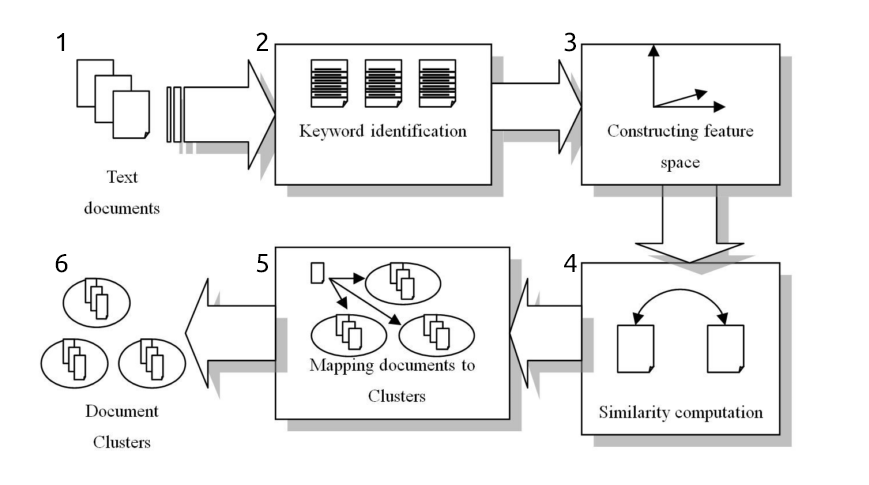
\includegraphics[width=12cm]{images/1_Text_Clustering_Main_Framwork.png}
  \end{center}
  \caption{ Text Clustering Main Framework from~\citet{Dozono2012} }
  \label{fig:1_Text_Clustering_Main_Framwork}
\end{figure}
In the first, step a data set must be provided in order to cluster the documents. 
The second step is where non relevant words are removed from the documents, which greatly improves clustering quality~\cite{Kang2003}. Another way to extract keywords is to differentiate text features by analyzing the document corpora. For example if the dataset is composed from HTML or XML documents it is possible to identify more relevant features due to the characteristics of the document syntaxe.
The fourth step is characterized by converting the keywords of each document into vectors, the most common model used for this task is VSM (Vector Space Model). In VSM, each vector dimension means one detected keyword and each document is represented by the vector of keywords in the feature space. This process an is described in Figure ~\ref{fig:2_svm}.

\begin{figure}
  \begin{center}
    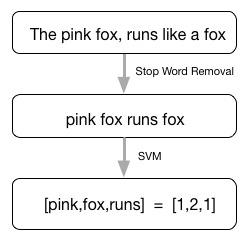
\includegraphics[width=5cm]{images/2_svm.jpg}
  \end{center}
  \caption{ Stop word removal and transformation to Vector Space Model }
  \label{fig:2_svm}
\end{figure}


There many clustering algorithms. K-means works by randomly selecting k documents as the cluster centroids, then assigning each document to the nearest centroid, and finally recalculate the centroid with new added documents. 

\section{The Self-Organizing Map} 
\label{sec:the_self_organizing_map}

The Self-organinzing map, or SOM, is a kind of recurrent artificial neural network that has the desired property of topology preservation which mimics the way the cortex of highly developed animals brains work.

As \citet{Bacao2005} describes, the basic idea behind SOM is to map the data patterns into an n-dimensional grid of neurons or units. That grid is also know as the output space, as opposed to the initial space also called input space, where the input patterns are. Both spaces can be seen in Figure~\ref{fig:5_neighbours_converge}.

SOMs work similar to the way that is thought that the human brain works. By having a set of neurons that through learning experience specialize in the identification of certain types of patterns. These neurons are responsible for categorizing the input patterns for which they are responsible to identify. Nearby neurons will be organized by similarity which will cause that similar patterns will activate similar areas of the SOM.
With a topology preserving mapping, SOM organizes the information spatially where similar concepts are mapped to adjacent areas. The topology is preserved in a sense that, as far as possible, neighborhoods are preserved through the mapping process.
Neurons are displayed in an N dimensional grid, generally rectangular, but other structures are possible, such as hexagonal or octagonal.  The grid of neurons, also called output space, can be divided in neighborhoods, where neurons responsible for the same kind of input reside.
In SOM, neurons will have the same amount of coefficients as the input patterns and can be represented as vectors through the VSM model described earlier in Section ~\ref{sub:clustering}.

Before describing the algorithm it is important to define two key aspects of the SOM, the learning rate and quantization error. The learning rate is a function that will be decreased in order to converge to zero, it will be applied to winning neurons and their neighbors in order for them to move toward the corresponding input pattern. Quantization Error is the distance between a given input pattern and the associated winning neuron, it describes how well neurons represent the input pattern. The radius of the neighborhood around the winner neuron is particularly relevant to the topology of the SOM, deeply affecting the unfolding of the output space as stated by \citep{Bacao2005}.
\par
The learning phase is characterized by the training algorithm, which works the following way:
\begin{itemize}
  \item Neurons can be initialized randomly or it is possible to select a specific initialization.
  \item Given an input pattern, calculate the distance between the input pattern and every neuron on the network.
  \item The winning neuron will be the closest neuron to the input pattern.
  \item The neuron will move towards the data pattern at a given learning rate, in order to improve his representation as can be seen in Figure~\ref{fig:4_wining_neuron_converge}.
  \item Neighbor neurons will also improve their representation in order to keep the network progressively organized as can be seen in Figure~\ref{fig:5_neighbours_converge}.
\end{itemize}

\begin{figure}
  \begin{center}
    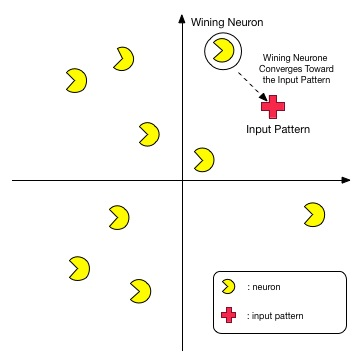
\includegraphics[width=5cm]{images/4_wining_neuron_converge.jpg}
  \end{center}
  \caption{ Winning neuron converging at learning rate }
  \label{fig:4_wining_neuron_converge}
\end{figure}

\begin{figure}
  \begin{center}
    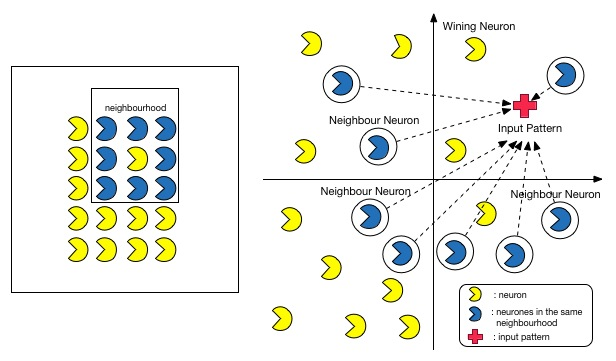
\includegraphics[width=12cm]{images/5_neighbours_converge.jpg}
  \end{center}
  \caption{ On the left the output space neighbor, on the right the neighbors of the winning neuron converging }
  \label{fig:5_neighbours_converge}
\end{figure}

After the algorithm converges, the prediction phase starts. On the prediction phase new input patterns can be quickly assigned to the SOM, without need to apply the learning rate to the winning neuron and his neighbors. Thus it very easy and fast to classify new data now.

In order to visually interpret the result of the SOM U-matrices may be used as stated by ~\citep{Bacao2005}. The U-matrix is a representation of the SOM in which distances, in the input space between neurons is represented using a gray scale.

The advantages of using SOM is data noise immunity, easy to visualize the data, and parallel processing~\cite{Liu2012b}.
 

\fancychapter{State of the art}
This section provides insight of work done in several research areas that are related to the project. In section ~\ref{sec:self_organizing_maps}, work done using \ac{SOM} maps will be described. Section ~\ref{sec:topic_detection_on_twitter} and~\ref{sec:data_mining_in_twitter_} are dedicated to data clustering and to data mining specifically on Twitter~\footnote{http://www.twitter.com}.

\section{Self-Organizing Maps} 
\label{sec:self_organizing_maps}
\ac{SOM} are used in a wide area of applications, from authentication systems~\cite{Dozono2012} through network intrusion detection~\cite{intrusion_som} and speech recognition and analysis~\cite{phonetic_typewiter}. In this section we highlight some of their applications.

\subsection{The Geo-SOM} 
\label{sub:types_of_soms}
The Geo-SOM, by~\citet{Bacao2005}, applies the first law of geography “Everything is related to everything else, but near things are more related than distant things."~\cite{citeulike:612692} to the \ac{SOM} algorithm. In this case, the winning neuron is chosen in a radius defined by the geographic-coordinates of the data, forcing units that are close geographically to be close in the output space.

The algorithm works by defining a variable $k$ which is used as a "geographical tolerance" that forces the winning neuron to be geographically near the input pattern. When $k=0$, the winning neuron is forced to be the unit geographically closest to the input data, whilst $k$ increases, the tolerance for data with further geographic coordinates, increases as well. $k$ is a geographic radius applied in the output space. When the radius exceeds the size of the output space, every unit is eligible to be the winning neuron, and therefor, we have a regular \ac{SOM}.

The selection of the winning neuron is done in two steps. First, geographic neurons inside the tolerance $k$ with the input data as a center are selected. Only after that, comparisons are made with the rest of data present in the input data. The representation of the Geo-SOM can be seen in Figure~\ref{fig:geo_som}, where the units considered for the best match are defined by a sort of geographic radius defined by $k$, whilst in the original \ac{SOM}, the winning neuron could have been any of the units presented on the figure.

The Geo-SOM approach to the alteration of the default \ac{SOM} algorithm is specially interesting due to the fact that this thesis objective is also to give relevance to data patterns that are not located in the same space as the trained data. In a way, what we are trying to achieve is similar to the work by~\citet{Bacao2005} but changing the geographic relevance in data by a social relevance.
\begin{figure}[tb]
  \begin{center}
    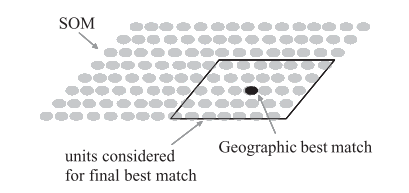
\includegraphics[]{images/6_geo-som.png}
  \end{center}
  \caption{Geo-SOM structure, where the units considered to be the winning neuron are constrained by the geographic coordinates of the data, from~\citet{Bacao2005}}
  \label{fig:geo_som}
\end{figure}

\subsection{Detecting Hidden Patterns on Twitter Usage} 
\label{sub:detecting_hidden_patterns_on_twitter_usage}
Cheon and Lee~\citep{Cheong2010} analyzed hidden patterns in the usage of twitter. In their study, they started by collecting data from the twitter API of different kinds of topics like "2009 Iran Election" and "iPhone 3.0 OS launch". They made multi level signal extraction, not only from information directly present on the tweet, but also by cross referencing with other social websites and with the twitter user profile information. The signals retrieved from the social network can be seen in Table ~\ref{tab:twitter_signals}.

\begin{table}[H]
  \caption{Twitter Signals}
  \label{tab:twitter_signals}
  \begin{center}
    \begin{tabular}{|l|}
      \hline
      \textbf{Twitt Corpus}  \\
      \hline
      Tweet Size \\
      \hline
      Replies \\
      \hline
      Re-tweets \\
      \hline
      Hashtags  \\
      \hline
      \specialcell{Presence of URIs and \\ Type of linked content} \\
      \hline
      Type of Device   \\
      \hline
      Tweet Location  \\
      \hline                 
      \hline                 
      \textbf{Twitter Profile} \\ 
      \hline
      Account Age   \\
      \hline
      Gender     \\
      \hline
      Country \\    
      \hline
      frequency of posts \\
      \hline
      Friends to followers ratio \\ 
      \hline
      Number of  customizations \\   
      \hline
      \hline
      \textbf{External Sources} \\
      \hline
      Other Social Network Accounts   \\
      \hline
      Type of website\\ 
      \hline
    \end{tabular}
  \end{center}
\end{table}

\textcolor{red}{Parece me interessante descrever quais as caracteristicas diferenciadoras dos clusters.}
By applying a \ac{SOM}, they could find four demographical clusters during the Iran 2009 Election. The first cluster was characterized by young web-based Iranians, with twitter accounts not older than three months with a high frequency of replies. The second cluster was mainly compound of web users from Iran accounts older that three months. The third cluster had Iranian users with mobile clients with large texts clearly trying to raise awareness. The fourth and final cluster represented the users around the world trying to raise awareness about the issue by sharing tweets with URIs.
Looking at their analysis about the topic "2009 Iranian Election", it is clear to see that it was possible to describe the type of users represented in the social network and the way they interact with it.

On the iPhone 3.0 OS launch, it was possible to find three main clusters. The first cluster was characterized by male users, accounts older than 90 days, coming from countries where the iPhone is marketed, with high adoption of social media clearly representing the target market of the iPhone or its customers. The second cluster had new accounts with higher rate of followers to followees, high frequency of posts per day, presence of URI linking to technology blogs or websites, no country or gender specified meaning that this cluster was clearly composed by news aggregators and technological news websites. Inside the second cluster, there was a sub-cluster of Japanese users which represents the high rate of iPhone adoption in Japan. Finally, the third cluster was clearly spammer accounts that where eventually deleted after a couple of months, characterized by popular social connections, posting more than fifty tweets a day with external URIs and the accounts were not older than a day or so.

In conclusion, it was possible to detect Twitter usage patterns, and specifically, detect spammers before they were banned from the social network. 

\subsection{WEBSOM}
\label{sub:websom}
\citet{honkelawebsom} developed a new approach to automatically order arbitrary, free from textual, document collections, using two different SOMs. The first \ac{SOM} is called word category map and its used to find words that have similar meaning, while the second \ac{SOM}, called document map, is the one actually used to cluster the documents. 

The WEBSOM was not based on keywords and boolean expressions, instead, words with the same meaning are encoded in a word category map (Fig~\ref{chp3:img3}), where placement and frequency in documents is taken into account. This way it is possible to remove words with similar meaning --- greatly reducing the \ac{VSM} size  making it possible to train the document map in a scalable way.
                                                                                                          
\begin{figure}[htpb]
  \centering
  \subfigure[The word cathegory map, a SOM where word frequency and placement is used for encoding text]{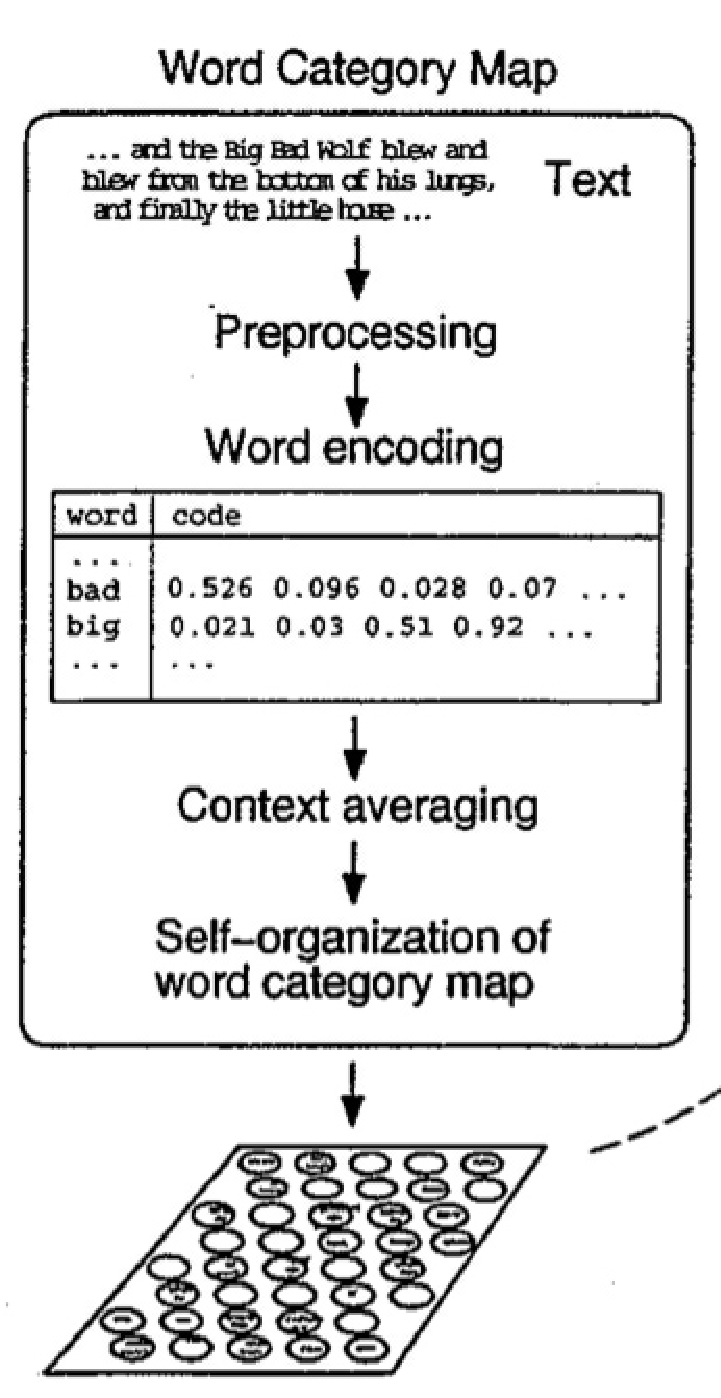
\includegraphics[scale=0.5]{./images/wordclusteringmap.pdf}\label{chp3:img3}}
  \hspace*{0.3cm}
  \subfigure[The document map, organized based on documents enconded with the word cathegory map.]{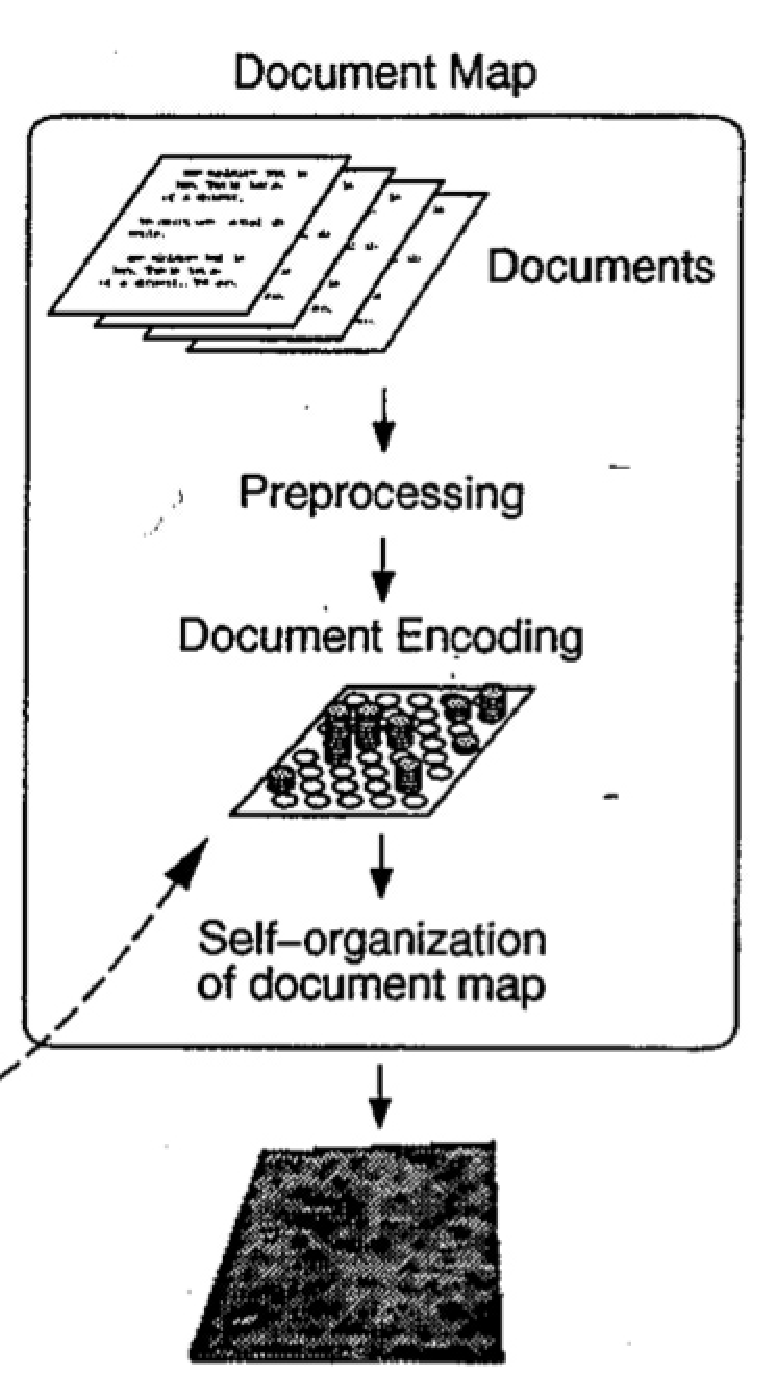
\includegraphics[scale=0.5]{./images/wordclusteringmapmap.pdf}\label{chp3:img4}}\\
  \caption{Basic architecture of the WEBSOM method, from~\cite{honkelawebsom}}
  \label{fig:websom}
\end{figure}
 
\section{Topic Detection and Tracking with Clustering} 
\label{sec:topic_detection_on_twitter}

~\citet{allan2002topic} defined \ac{TDT} as: “\ac{TDT} research begins with a constantly arriving stream of text from newswire and from automatic speech-to-text systems that are monitoring selected television, radio, Web broadcast news shows. Roughly speaking, the goal of \ac{TDT} is to break the text down into individual news stories, to monitor the stories for the events that have not been seen before, and to gather stories into groups that each discuss a single news topic".

Nowadays, due to the rapid adaptation of people to always be on-line, through the usage of cellphones on the move, desktops at work and even TV at home, the increase of user generated content has increased tremendously in latest years. In 2006, 35\% of on-line adults and 57\% of teenagers created content on the Internet \footnote{ Data source: http://www.pewinternet.org/Presentations/2006/UserGenerated-Content.aspx}, which in "Internet Years" was ages ago. 

The challenge of \ac{TDT} is evermore focused on online generated documents, and in new forms to be able to track and categorize all the information that is continuously being generated.
Many \ac{TDT} techniques have been proposed,  a significant amount of them rely on the \ac{TF-IDF}~\cite{Baeza-Yates:1999:MIR:553876}. Because tweets are very small, often with typos or slang words, and because the same tweet might be written in multiple languages, \ac{TF-IDF} is not particularly adequate for topic detection on twitter. In this subsection, we will take a look at multiple methods of topic detection in general, and also specifically on the Twitter social network.

\subsection{Topic and Trending Detection} 
\label{sub:real_time_topic_and_trending_detection}
%With amount of content increasing, new real-time and scalable algorithms are needed in order to make sense of all this data.
~\citet{Cataldi2010} proposed a new technique for emerging topic detection that permits real-time retrieval of the most emergent topics expressed by a community on Twitter. Their work applies the PageRank algorithm~\cite{Pagerank1998} to the users follower/followee relationship, in order to find the most influential users on the network. Then, the most trending topics are calculates, by relating social influence, word co-occurrence and time frame. In the end, an interface was created where it would be possible to navigate, through hot topics in a given time frame. Topic labeling was not automatic and was implicit by the time frame of an event.
%REMOVEDBYPAVEL
%, if two highly social events would occur in the same time frame with word relations the results could be interpreted as the same, for example if a political candidate would win the elections at the same of an important sports club would win a specific cup, the word \emph{win} could be trending at the same time for two different topics and due to high temporal dependency they could be interpreted as the same topic.

~\citet{Weng2010} also used the PageRank algorithm to find the most influential twitter users on a certain topic. However, using a different approach, they represent each twitter user as a bag of words comprising of all the tweets that they have posted, and applied \ac{LDA}~\cite{Blei2003} in order to find topics in which users are interested in. Finally, it was possible to prove that follower/followee relations on twitter are not just casual, but that people actually follow other people to whom they have some resemblance or common interest. This concept is called homophily and will be further explored on this thesis.

\section{Twitter Data Mining} 
\label{sec:data_mining_in_twitter_}
In this subsection, we will focus on work done on the Twitter social network in order to leverage insights on how the public data available from the website can be explored. 

\subsection{Tweets Implicit Data} 
\label{sub:the_tweet}
Tweet retrieval and analysis is a double edged problem. On one side, the tweet is really small, which makes it almost impossible to retrieve any actual sense from it. On the other hand, the amount of tweets generated per day is around 140 million\footnote{https://blog.twitter.com/2011/numbers}, which means that it is very hard to do a deep analysis of the semantics and content of individual tweet, and that only the more appropriate signals should be evaluated.
For this reason, \citet{Tao2012} evaluated how the multiple signals that could be retrieved, directly or indirectly, from the tweet corpus could mean that a tweet is relevant for a determined topic. In their work, they present premises that seem intuitively true and proves they actually are relevant through a comparison of multiple precision and recall values. Their results on feature comparison are summarized in Table~\ref{tab:tao_table}. The first column consists of all the made hypothesis categorized by type, and the second column tells if the data used actually influenced in precision and recall results. \citet{Tao2012} also compared results, of topic characteristics, concluding that distinction between local and global events as well as temporal persistence proved to not be relevant on relevance prediction.

\begin{table}[tb]
  \caption{~\citet{Tao2012} tweet characteristics hypothesis versus influence}
  \label{tab:tao_table}
  \begin{tabularx}{\textwidth}{|X|l|}
  \hline
  \textbf{Hypotheses} & \textbf{Influence of Features} \\
  \hline
  \hline

  {\bf Syntatical} &  \\
  \hline
  Tweets that contain hashtags are more likely to be relevant than tweets that don't & Not Important \\
  \hline
  Tweets that contain an URI are more relevant that tweets that don't  &Important \\
  \hline
  Tweets that are replies to other tweets are less relevant & Important \\
  \hline
  The longer the tweet is the more relevant it is & Not Important\\
  \hline
  \hline

  {\bf Semantic}  &  \\
  \hline
  
  The more the number of entities the more relevant a tweet is  & Important \\
  \hline
  Different types of entities are of can have different amount of interest to a give topic  & Important \\
  \hline
  The greater the diversity of concepts mentions in a tweet the more likely for it to be relevant & Important \\
  \hline
  The relevance of a tweet is determined buy its polarity & Important \\
  \hline
  \hline

  {\bf Contextual} &  \\
  \hline
  The lower the temporal distance between a query and the creation of a tweet the more relevant the tweet is  & Not Important \\
  \hline
  The more the number of tweets created by a user the more relevant one of his tweets will be & Not Important \\
  \hline
  \end{tabularx}
\end{table}

~\citet{McCreadie2013} also approached the issue of having very little content on tweets in order to categorize them, and tried to solve the problem by applying the content of linked URIs into the tweet body in order to improve precision and recall. The best fitting approach was using Field-Based weighting, where for each tweet a new document is created, which contains two fields: the terms in the tweet and the terms in the linked document. 
Afterwards a learning to rank algorithm called PL2F~\cite{macdonald2008} is used against the dataset from "Trec Microblog2011" in order to find the best weighting. 
With this model they were able to improve precision in an order of 0.9, over only analyzing the text contained in the tweets. 

\subsection{Tweeter Natural Language Processing}
\label{sub:tweeter_natural_language_processing}
Using standart \ac{NLP} tools on tweets has been extremely unreliable, due to the fact that microbloging text tends to be full of abbreviations, emojis and smiles . Recently, ~\citet{owoputi13improvedparth} published a \ac{NLP} library, specific for twitter. As shown in Figure~\ref{fig:nlp}, ARK Tweet \ac{NLP} can tag words that are only used in social networks. The tagger was built using maximum entropy Markov model, where a tag is assigned to a word based on the entire tweet text, and the tag assigned to the word to its left. ~\citet{owoputi13improvedparth} state that the tagger has a 93.2\% accuracy. 
By using \ac{NLP} tools, it is possible to reduce the dimension of \ac{VSM} space by only choosing words that are relevant, like common nouns, hashtags and proper nouns. This will not only yield better results by removing tweets that have no content, and therefor, cannot be categorized, but will also increase performance during training due to the reduced dimensions caused by less use of words.
\begin{figure}[htpb]
  \centering
  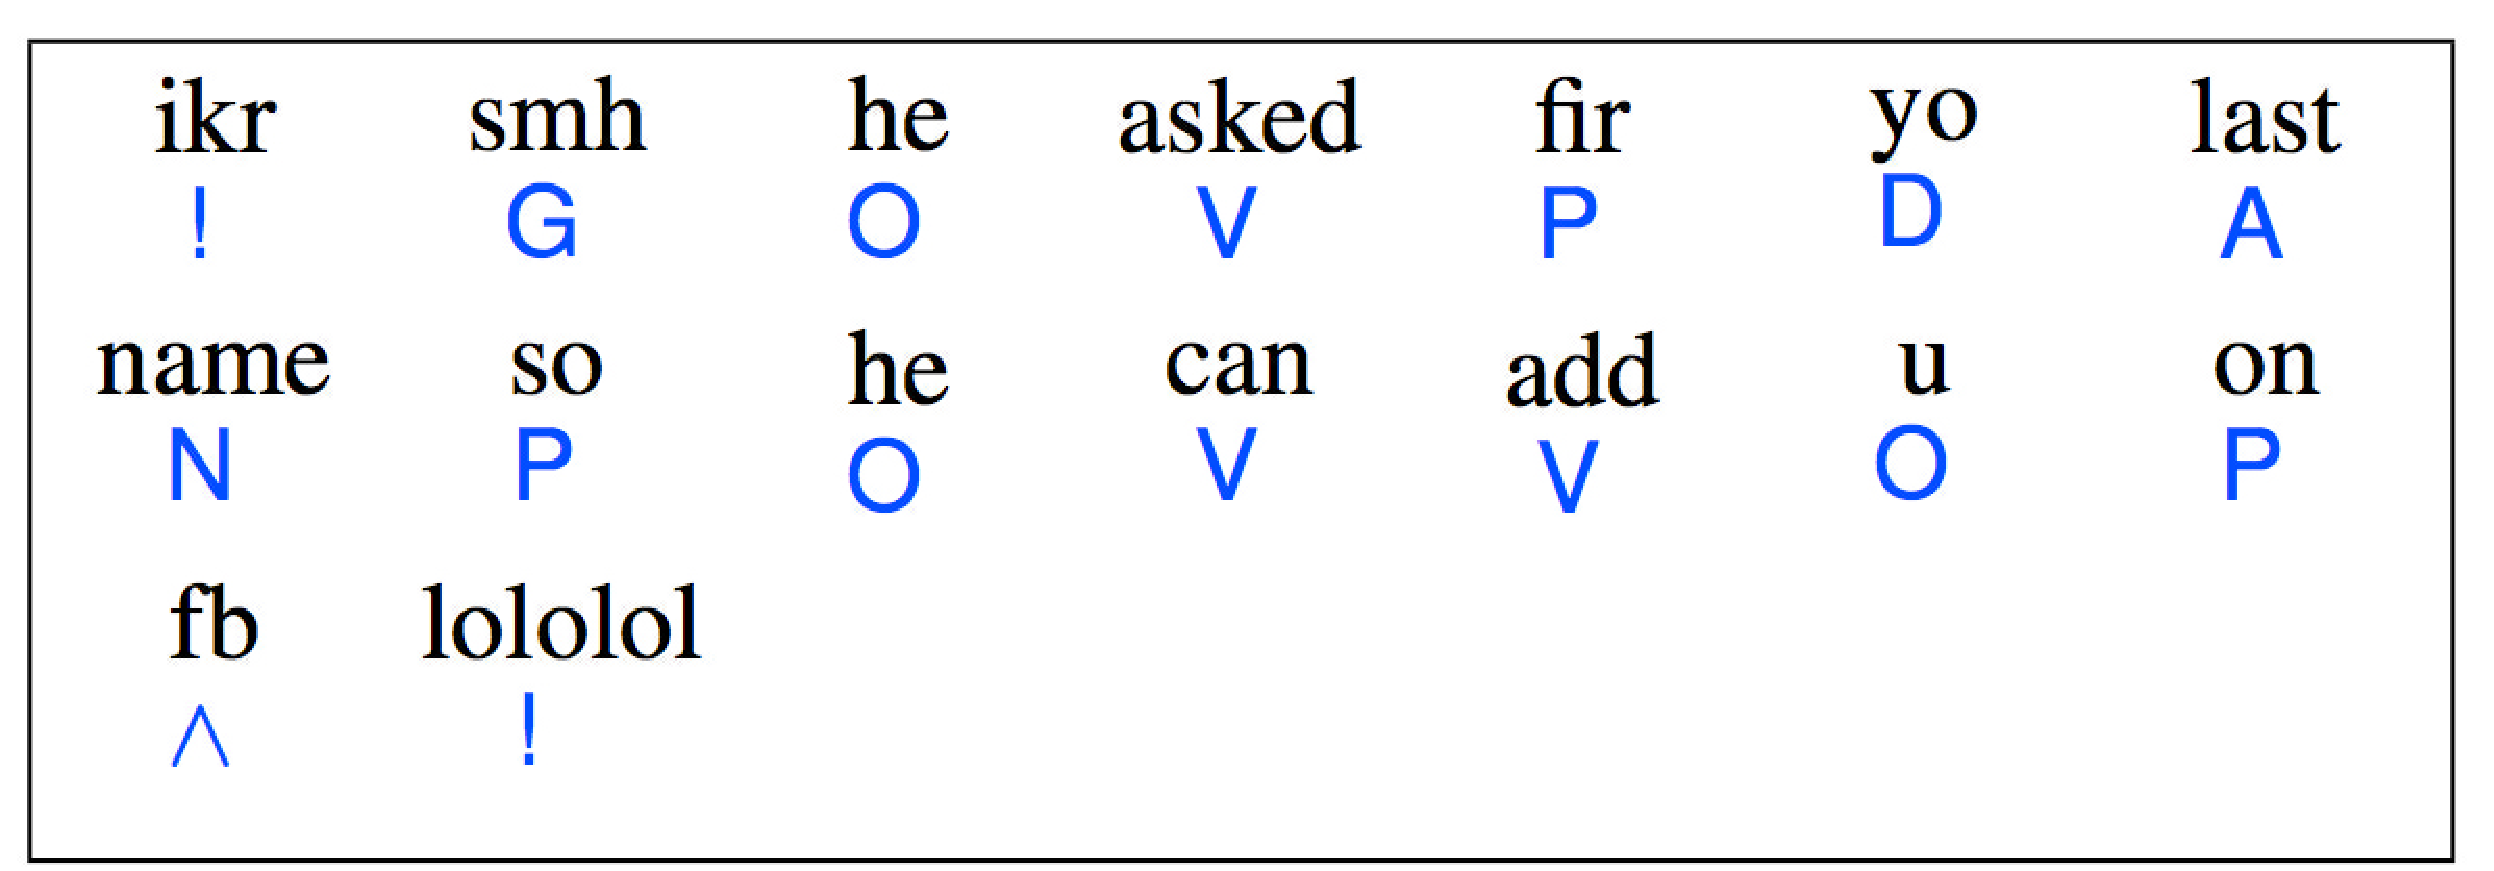
\includegraphics[width=0.6\linewidth]{./images/nlp.pdf}
  \caption{Tweet automatically tagged with ARK Tweet NLP. ! stands for interjection, while V stands for verbs and D for determiner. The full table of tags can be found in~\cite{owoputi13improvedparth}.}
  \label{fig:nlp}
\end{figure}

\subsection{Rapidly Changing Trends} 
\label{sub:real_time_}
Due to the real time nature of Twitter, using typical retrieval model, that relies on term frequency models like Okapi BM25 or language modeling cannot be applied, as stated by~\citet{Lin2012}. The study of topic endurance on the social network proved that topics are presented in bursts of queries and mentions. In addition the typical usage of twitter for search is not the same of Google. When users are searching on twitter, they want to find out what is happening in that moment, meaning that classification techniques based on past events cannot respond this kind of problem. As stated by~\citet{Lin2012}, this problem has not yet been solved at Twitter (or anywhere else at the time of writing this report), and issues a new kind of data analysis approach that was not taken into consideration in the past. 

This effect of rapidly changing topics and queries based on real time events was named "Churn", and can be clearly seen in Figure ~\ref{fig:churn}.

By including social features into clustering algorithms, it might be possible to discover interesting rising topics to a specific specific user, by categorizing them through a trained \ac{SOM}.

\begin{figure}[tb]
  \begin{center}
    \noindent\makebox[\textwidth]{
      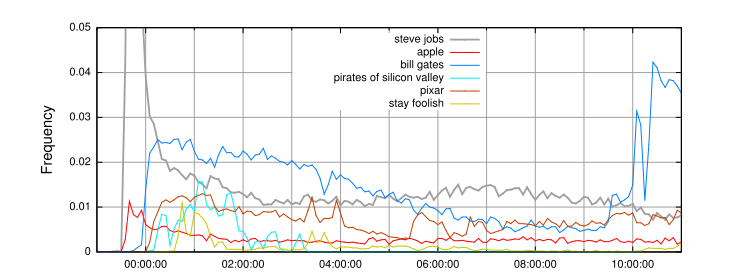
\includegraphics[width=13cm]{images/7_churn.png}
    }
  \end{center}
  \caption{The Churn effect: Frequencies of queries related to Steve Jobs death over a 12 hour period in 5-minute intervals, normalized to the total number of queries in the interval. At its peak, the query “steve jobs” reaches 0.15 (15\% of the query stream); Graph taken from~\cite{Lin2012}}
  \label{fig:churn}
\end{figure}


\section{Summary}
%TODO Sumarize the state of the art
Ending section summarizing the chapter is typically a good idea.

Ensure that the next chapter starts in a odd page
\cleardoublepage 

\fancychapter{Clustering Tweets with Self Organizing Maps}
\label{ch:clustering_tweets}

\section{Twitter Data}
\label{sec:crawling_twitter}
Twitter is a social network website and mobile app, where users are able to share what's on their mind with less than 140 characters. Due to its limitations, twitter users started to adopt their own kind of language on the social network, sharing shortened \ac{URL}, and tagging topics with a word preceded with an hashtag -- \# -- became so popular, that it was eventually implemented into twitter itself. Nowadays it is possible to monitor events through hashtags selections and links shared on the mobile app are automatically shortened.   

With the rise of smartphones and decent prices for mobile Internet access, and people becoming always online, GPS coordinates were also added to tweets. In fact, a tweet nowadays has a massive amount of information, as can be seen in Figure~\ref{fig:json_tweet}.


There are two main ways to gather data from twitter: Crawl twitter HTML pages and scrap the intended information, access through the twitter API.

Crawling web pages is done through the analysis of HTML documents generated by twitter servers. Due to specific semantic rules, it is possible to gather almost all information that is possible to have access through the twitter API. Even though writing an HTML crawler is not particularly complex, specially through the usage of open source tools like nokogiri \footnote{http://www.nokogiri.org/} or beautiful soup \footnote{http://www.crummy.com/software/BeautifulSoup/}, Twitter specifically asks to not be crawled in some parts of their \ac{URL}, as can be seen in Figure~\ref{fig:twitterrobots}. 

Basically, the restrictions that twitter asks on his robots.txt, only allows for search results, and hashtag searches to be monitored, which is pretty limiting.

\begin{figure}[htpb]
  \centering
  \begin{boxedverbatim}
  # Every bot that might possibly read and respect this file.
  User-agent: *
  Allow: /?lang=
  Allow: /hashtag/*?src=
  Allow: /search?q=%23
  Disallow: /search/realtime
  Disallow: /search/users
  Disallow: /search/*/grid

  Disallow: /*?
  Disallow: /*/followers
  Disallow: /*/following

  Disallow: /account/not_my_account

  Disallow: /oauth
  Disallow: /1/oauth
  \end{boxedverbatim}
  \caption{Twitter robots.txt piece where it is possible to see what should and shouldn't be crawled.}
  \label{fig:twitterrobots}
\end{figure}

Since version 1.1, authentication is required in order to access twitter through their API. The authentication mechanism, is used to limit the amount of information users can gather from twitter. 
The API itself is divided in the streaming -- used for subscribing directly to twitter public, user or site streams --  and REST -- used for programmatic access to read and write to the twitter API.  

The streaming API is extremely useful for building datasets based on keywords, searches and entities. A huge amount of tweets can be collected without hitting rate limits, since their API default level lets an endpoint track up to 400 words, and 5000 user ids. As long as the amount of tweets streamed to the endpoint doesn't  surpass the 1\% of the total amount of tweets Twitter is currently streaming. Although, if some wrong terms are monitored, the amount of spam crawled can be huge, specially when monitoring public entities or trending hashtags. 

The REST API can be used to get all information that is available on twitter by the time the request is sent. REST API limits are much greater than the ones applied at the streaming API. The basic rules are 15 minutes windows per endpoint where 15 requests can be made. There are some exceptions to these rules and those can be found on twitter documentation \footnote{https://dev.twitter.com/rest/public}.

\begin{figure}
  \begin{center}
    \begin{lstlisting}[language=json,firstnumber=1]
{ 
  "_id" : { "$oid" : "4fa14bc97e5617025fb14787" },
  "text" : "RT @FastCoDesign: A Paintbrush That Works On The iPad http://t.co/eWjEZAga (@sensubrushman)",
  "id_str" : "197701817864421376", 
  "coordinates" : null, 
  "in_reply_to_screen_name" : null, 
  "in_reply_to_user_id" : null,
  "possibly_sensitive" : false, 
  "favorited" : false, 
  "in_reply_to_status_id" : null, 
  "source" : "<a href=\"http://www.flipboard.com\" rel=\"nofollow\">Flipboard</a>", 
  "possibly_sensitive_editable" : true, 
  "contributors" : null, 
  "retweet_count" : 0, 
  "truncated" : false,
  "in_reply_to_status_id_str" : null,
  "geo" : null,
  "in_reply_to_user_id_str" : null,
  "entities" : { Enteties Object },
  "user" : { User object },
  "retweeted" : false,
  "id" : 197701817864421376,
  "place" : null,
  "created_at" : "Wed May 02 14:59:21 +0000 2012" }

    \end{lstlisting}
  \end{center}
  \caption{\ac{JSON} representation of a Tweet.}
  \label{fig:json_tweet}
\end{figure}



Due to the amount of specificity allowed by the REST API, it is better suited to create datasets that mimic the way twitter data is interconnected, like getting users and their followers, as well as their tweets.

\subsection{Crawling Twitter for Social Relations}
\label{sub:crawling_twitter_for_social_relations}
While researching ways to use \ac{SOM} as a way to find clusters of topics on twitter, we presented some enhancements to the algorithm, which integrates the social network behind the authors of the tweets in the clustering process. In order to analyze socially linked data, a socially linked dataset is needed, and therefor a crawler that stores social connections between users must be implemented.   

Given the fact that social relations were required, we opted for making a crawler based on the REST API. Due to the fact that twitter API rate limits would be achieved with some ease, the crawler should be prepared to achieve this maximum amount of requests per 15 minute window and wait until it can crawl again. 

Also, at a given time, the crawler should be able to serialize it state in order to able to resume crawling in case it has to stop at any given worldly circumstances. 

\section{SOM}

\subsection{Clustering Tweets}
\label{sub:clustering_tweets}

In order to use \ac{SOM} to cluster tweets, first the tweets need to be converted into \ac{VSM}. Given the fact that tweets are often misspelled, with slang words and are written in multiple languages, the \ac{VSM} tends to become pretty large with relative ease. 

In order to reduce the amount of different words that could have the same meaning, or no meaning at all, the following rules were applied:

\begin{itemize}
  \item Only English tweets were used during clustering.
  \item \ac{URL} are removed. Since most of them are minimized, little information can be taken from them without domain translations.
  \item Numbers are removed.
  \item All letters are down cased.
  \item Runs of a character are replaced by a single character.
  \item Words smaller than 3 chars are discarded.
  \item Stop words are removed. 
  \item The tweet text is stemmed.
\end{itemize}

By applying these rules, the \ac{VSM} is greatly reduced without destroying major relevant words. More information about \ac{VSM} reduction can be found on Sub-chapter~\ref{sub:reducing_som_vector_size}. A visual application of these methods can be seen in Figure~\ref{fig:string_reduction}.
\begin{figure}[htpb]
  \centering
  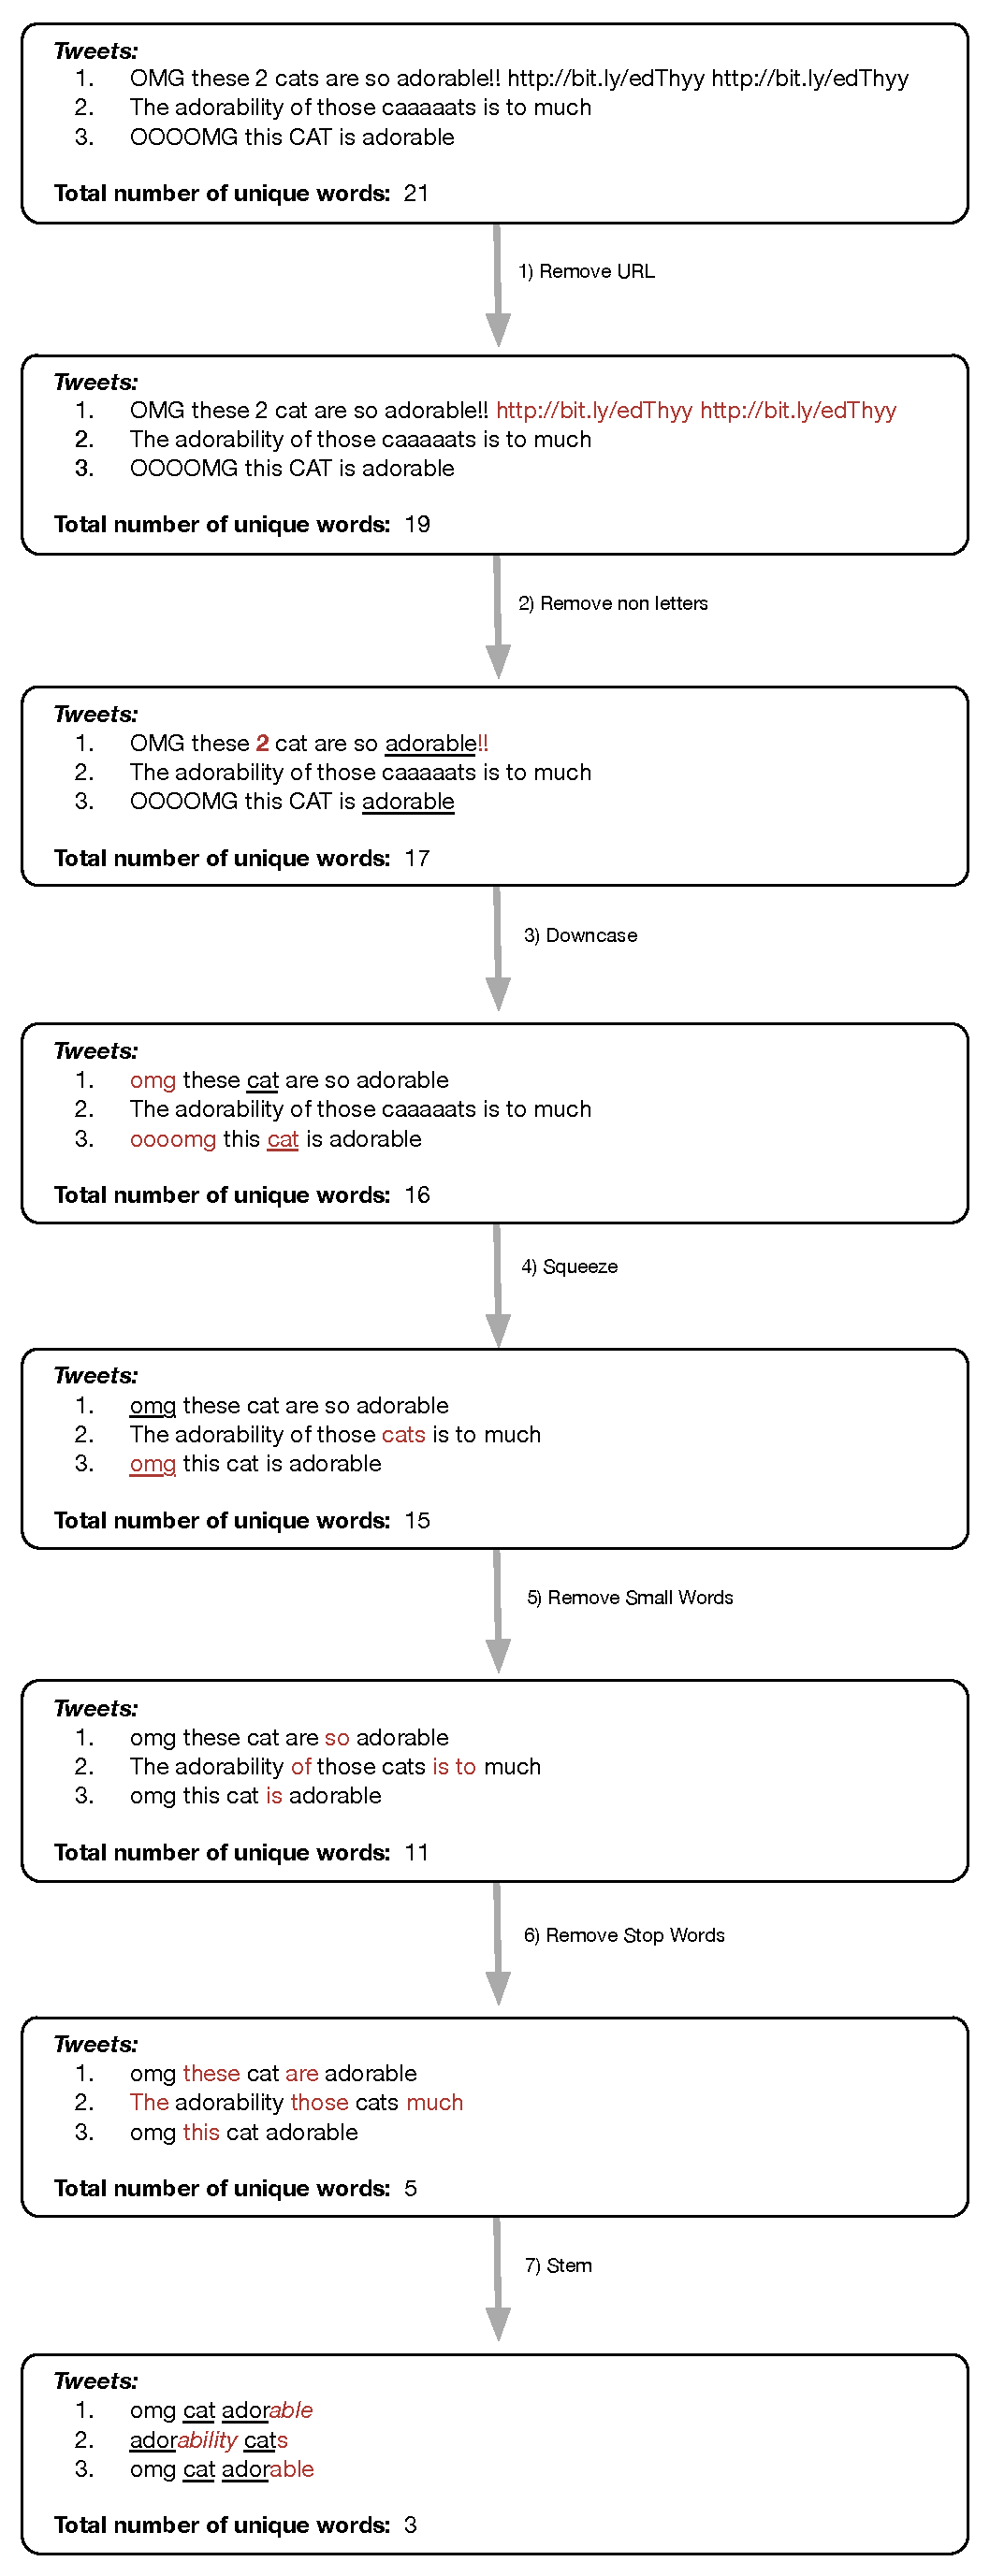
\includegraphics[width=0.5\linewidth]{./images/string_reduction.pdf}
  \caption{Reducing the number of unique words on three tweets about cats. Text in red represents letters removed. Underlined text represents words that due to text transformation became equal.}
  \label{fig:string_reduction}
\end{figure}

Since tweets are very small and have an average of only 10 to 14 words, there is no need to store term frequency on the \ac{VSM}, and therefor only a binary count is made.

\ac{NLP} techniques such as the one described on Subsection~\ref{sub:tweeter_natural_language_processing} can be used in conduction of the method described above for even a more efficient \ac{VSM} reduction. In order to accomplish this, first we need to run the \ac{NLP} on the dataset and specify what kind of tags we want to use. Then, we run the string reduction techniques described above on the words tagged by the \ac{NLP}, these words will then be used to create the \ac{VSM} where each word represents on column. This process can be seen in Figure~\ref{fig:string_nlp}.
\begin{figure}[htpb]
  \centering
  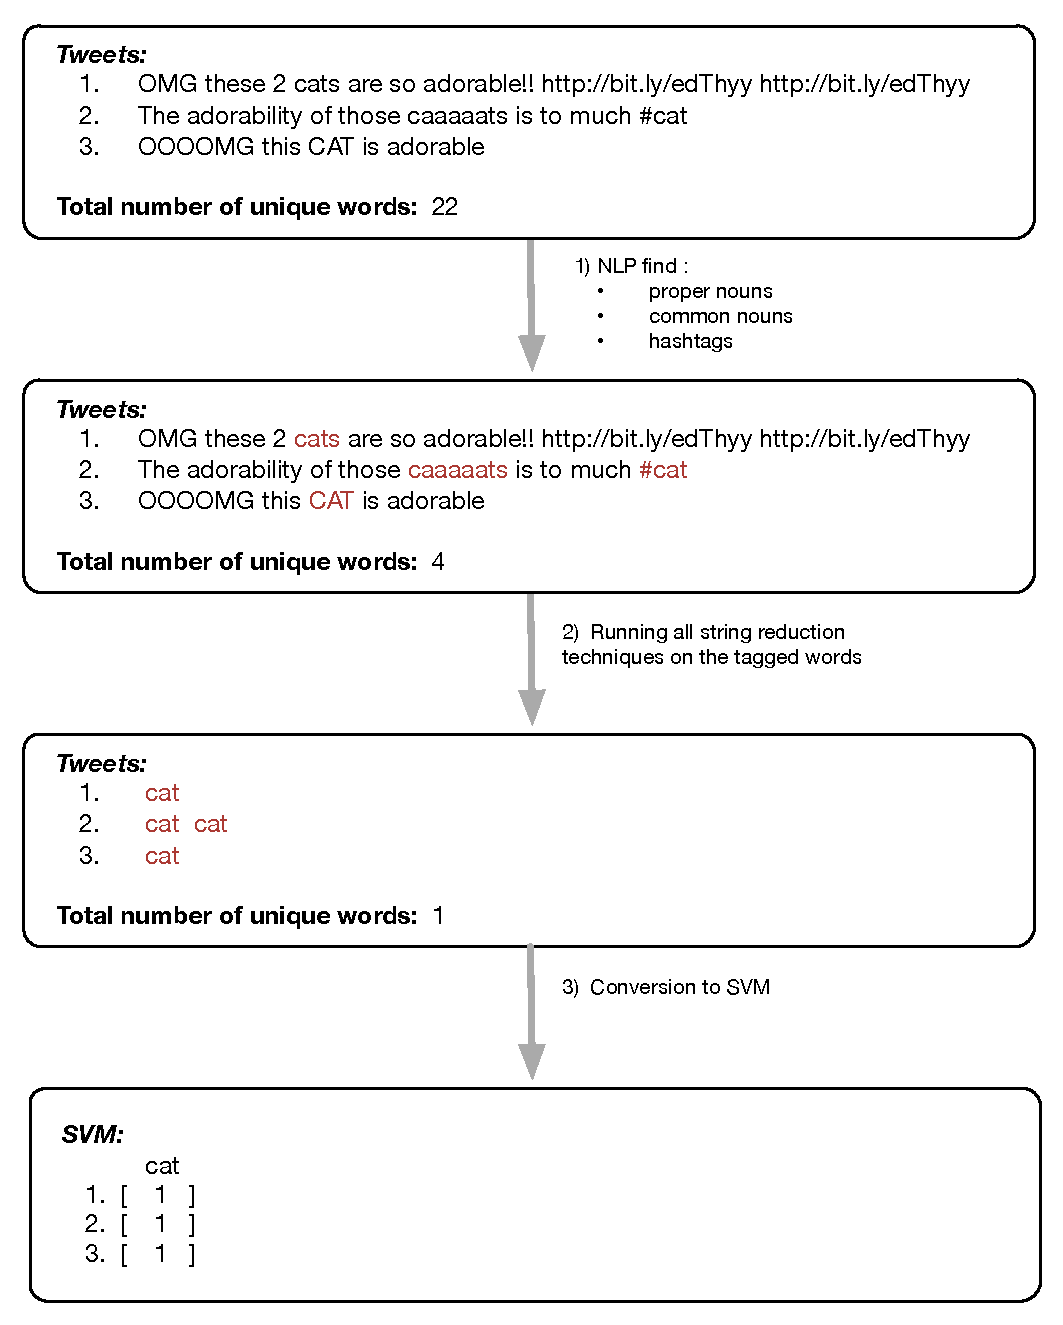
\includegraphics[width=0.8\linewidth]{./images/string_reduction_nlp.pdf}
  \caption{Using NLP with string reduction techniques to reduce the VSM size}
  \label{fig:string_nlp}
\end{figure}

Converting tweets from text to \ac{VSM} can be done in two different approaches. The first one is the cumulative approach, where the \ac{VSM} is being built at the same time that the tweets are read, new terms are added as columns to the \ac{VSM} as soon as they are found. The second way relies on scanning all words present in the dataset in order to first build the \ac{VSM}, then iterate through all tweets and mark them as ones and zeros if they occur in the tweet text. 


After the \ac{VSM} is filled with tweets, it can be feed to the \ac{SOM} and therefor training can start. It is important to notice though, since a destructive process was done to minimize the size of the \ac{VSM} some extra mechanisms must be implemented in order for the tweets to be humanly readable after training.



\subsection{Extensible SOM Library}
\label{sub:extensible_som_library}

When researching ways to extend the \ac{SOM} algorithm, in order to add social features to the learning process. We found that the number of \ac{SOM} libraries was not very expense. Even though, programing languages often used in \ac{ML} and Data Mining, such as Python or C++, have their own implementation of the \ac{SOM} algorithm. We've found that most of these libraries are made in such a way to be extremely fast, in order to take as much advantage from the hardware they are running on as possible. They often lack the modularity needed to adapt the \ac{SOM} algorithm to specific problems.

The \ac{SOM} algorithm has been changed many times in order to better categorize data with specific features. For example, the previously described in Subsection~\ref{sub:types_of_soms} Geo-\ac{SOM}, the Growing Hierarchical \ac{SOM}~\cite[]{1058070}, the time adaptive \ac{SOM}~\cite[]{1187438}, the Ontological \ac{SOM}~\cite[]{5446427}, and the list goes on\dots  

In order to create the homophilic \ac{SOM}, described in Section~\ref{sec:algorithm_changes} we first created a \ac{SOM} framework that is easy to extend due to be fully object oriented, scripted --- even though it can be compiled to run on the JVM --- and without C extensions.



\section{Homophilic SOM Definition}
\label{sec:algorithm_changes}
The default \ac{SOM} algorithm has no idea whatsoever of the social connections between the tweets, it simply looks at the binary vectors that represent sentences and assigns it to the most similar neuron.

In order to better categorize socially connected data, we propose some alterations to the \ac{SOM} algorithm in order to make it aware of the social connections between the tweets, and therefor, better represent the homophilic behavior present on social networks.

\subsection{Output Space}
\label{sub:output_space}
The output space is the zone on the \ac{SOM} algorithm where the neurons reside. It works like a cortex where neurons are scattered in a geometric fashion, generally a square. The output space is generally initialized with random values, with a relatively high learning rate, and also a relatively high number of epochs. The algorithm is made this way in order to be able to identify any type of data that can be represented as vectors.

First, we will try to change the output space to better resemblance the social network. In order to do this, the squared grid that defines the output space was changed by the social network connections, and the neurons, are represented by a social network user. This changes are applied in the following way:
\begin{figure}[htpb]
  \centering
  \subfigure[The neighbourhood is defined by the relations of followers/followees between the winning neuron and the other neurons]{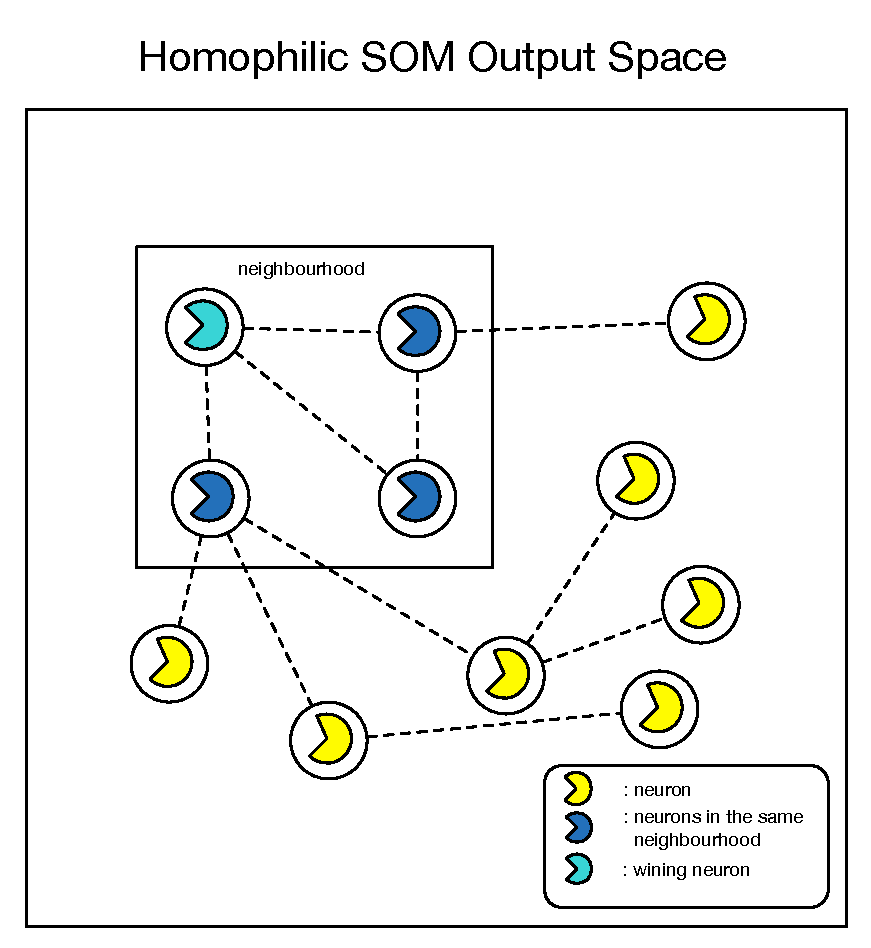
\includegraphics[scale=0.3]{./images/homophilic_outputspace.pdf}\label{chp3:homout}}
  \hspace*{0.5cm}
  \subfigure[Homophilic input space works in the same way as a normal input space]{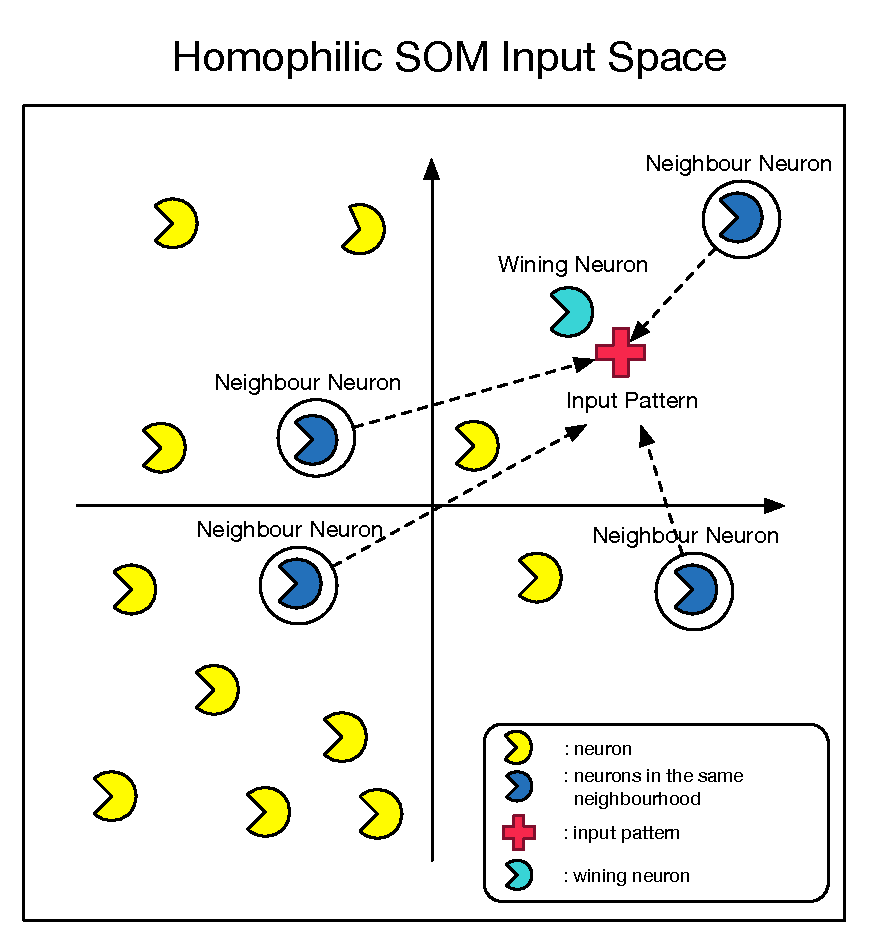
\includegraphics[scale=0.3]{./images/homophilic_input_space.pdf}\label{chp3:homin}}
  \label{fig:homo_in_out}
  \caption{ Homophilic SOM output and input space during the learning phase. }
\end{figure}
\begin{itemize}
  \item Each neuron is comprised of the text from all the tweets that he authored.
  \item Each neuron has a unique id, and stores the ids of his followers and followees that are present in the output space.
  \item During the learning phase, the radius will be defined as the maximum number of hops separating the winning neuron and followers/followees of followers/followees. 
  %\item Each neuron will cache followers/followees of a follower/followee to a specified depth level, for performance purposes. 
\end{itemize}


\subsection{Learning Phase}
\label{sub:learning_phase}
Like in the default \ac{SOM}, the learning phase is where the output space is trained in order to organize the input data into clusters. Since this algorithm is specific to categorize tweets using social network features, the learning rate, radius and number of epochs used can be greatly reduced in order for the algorithm to converge. The learning phase operates in the following way:

\begin{itemize}
  \item The distance between the input pattern and all the neurons is calculated. The neuron closest to the input pattern is considered the winning neuron.
  \item When the winning neuron is selected, it and its social neighbors within k hops, update their representations in the input space, and move closer to the input pattern. The Gaussian function (Func.~\ref{eq:gaussian}) is also used here. As a way for the neighbors that are closer to the winning neuron, be significantly more influenced by the input pattern, while the neurons further away are less influenced. 
  \item This process is repeated for a predefined number of epochs. In order for the algorithm to converge, whilst the number of epochs increases, the learning rate and number of hops that defines the neighborhood decreases.
\end{itemize}

Just like the default \ac{SOM} algorithm, after the map is trained, input patterns can be fast assign to the nearest neuron since the neuron positions in the output space are no longer updated.

\subsection{Visualizing Neuron Representation Quality}
\label{sub:visualizing_neuron_representation_quality}
The homophilic \ac{SOM} has an output space that doesn't relate to any kind of geometric figure, due to this fact, it is not possible to visualize the clusters formed using \ac{U-Matrix}. In order to solve this problem, we propose an alternative way to visualize \ac{SOM} that, instead of focusing on the distance between the neurons on the output space --- like the \ac{U-Matrix} ---, it focuses on the mean quantization error applied to each neuron and the input patterns it is representing. We named this method Q-Matrix ( Alg. \ref{alg:qmatrix} ) which stands for unified mean quantization error matrix.

\begin{figure}[h]
  \begin{algorithm}[H]
    \label{alg:umatrix}
    \DontPrintSemicolon
    \KwData{Input patterns $X = \{  \overrightarrow{x_1}$,\dots,$\overrightarrow{x_N}$ \}, Trainned neurons $W = \{  \overrightarrow{w_1}$,\dots,$\overrightarrow{w_N}$ \} }
    \KwResult{U-Matrix}
    \For{ $w_d = \overrightarrow{w_1}$ to $\overrightarrow{w_N}$ }{
      (NOTA: Nao sei muito bem como escrever isto numa formula matematica..) the average of all the distances between a neuron and all of the input patterns he represents
      }
      \caption{U-Matrix }
  \end{algorithm}
\end{figure}


The algorithm works in the following way: for each neuron in the grid, we find the quantization error between it and all the input patterns it represents. Afterwards, we calculate the average between all the quantization errors associated to the neuron, and add it to the Q-Matrix. After this process is applied to all neurons, all quantizations errors are converted to a color that is directly proportional to the amount of the mean quantization error. 

Due to the fact that each neuron is a cluster on the homophilic \ac{SOM}, the Q-Matrix algorithm lets you easily see which clusters have the lower quantization error, and therefor better match their input data. On the default \ac{SOM} algorithm, the Q-Matrix can be applied in order to easily visualize which neurons don't represent well their input patterns, being an extra tool to analyze training quality. An example of a Q-Matrix can be seen in Figure~\ref{fig:som_trqmatrix}.
\begin{figure}[htpb]
  \centering
  
\includegraphics[scale=2]{./images/som_training/2_quantmatrix.pdf}
  \caption{Q-Matrix calculated after 300 epochs of training a default \ac{SOM} algorithm to identify colors. By looking at the matrix it is very easy to see which neurons are not representing their associated input patterns well -- in black -- and in white the ones that have very little quantization error and therefor are good at representing their input patterns}
  \label{fig:som_trqmatrix}
\end{figure}


% \fancychapter{Implementation}
 %TODO how it was implemented
I have no idea what to write here\dots

\begin{figure}
\begin{boxedverbatim}
DefineGlobals
   clock   alias   clk
   reset   alias   rst
   max_latency     17
   feedback        0
   DefineInputs
      X   std_logic_vector(11 downto 0)
   EndInputs
   DefineOutputs
      Y   std_logic_vector(11 downto 0)
   EndOutputs
EndGlobals
\end{boxedverbatim}
\caption{An example code section.}
\label{chp4:img}
\end{figure}

Figure~\ref{chp4:img} shows an example of a \verb"\boxedverbatim" section. It allows to put blocks of code within a frame. I think makes a prettier printing.

\section{Summary}

An ending section summarizing the chapter, is typically a good idea.

% Ensure that the next chapter starts in a odd page
\cleardoublepage


\fancychapter{Evaluation Metrics}


\section{Clustering Tweets with Self-Organizing Maps}
\label{ch:clustering_tweets}

\subsection{Twitter Dataset}
\label{subsec:twitter_dataset}

Each tweet is comprised of multiple parameters. Figure~\ref{fig:json_tweet} shows how a tweet is represented in \ac{JSON} format. Inside the tweet there is also information about the user whom created the tweet, shown in Figure~\ref{fig:json_tweet_user} and entities shown in Figure~\ref{fig:tweet_enteties}.

As can be seen in Figure~\ref{fig:json_tweet_user} no information about the social relations of the user which emitted the tweet are present. Therefor in order to retrieve the social network in which a user is contained, it will be necessary to connect to the Twitter API. Crawling twitter is discussed in further depth in Chapter~\ref{chap:crawling_twitter}.  

\begin{figure}
  \begin{center}
    \begin{lstlisting}[language=json,firstnumber=1]
{ 
  "_id" : { "$oid" : "4fa14bc97e5617025fb14787" },
  "text" : "RT @FastCoDesign: A Paintbrush That Works On The iPad http://t.co/eWjEZAga (@sensubrushman)",
  "id_str" : "197701817864421376", 
  "coordinates" : null, 
  "in_reply_to_screen_name" : null, 
  "in_reply_to_user_id" : null,
  "possibly_sensitive" : false, 
  "favorited" : false, 
  "in_reply_to_status_id" : null, 
  "source" : "<a href=\"http://www.flipboard.com\" rel=\"nofollow\">Flipboard</a>", 
  "possibly_sensitive_editable" : true, 
  "contributors" : null, 
  "retweet_count" : 0, 
  "truncated" : false,
  "in_reply_to_status_id_str" : null,
  "geo" : null,
  "in_reply_to_user_id_str" : null,
  "entities" : { Enteties Object },
  "user" : { User object },
  "retweeted" : false,
  "id" : 197701817864421376,
  "place" : null,
  "created_at" : "Wed May 02 14:59:21 +0000 2012" }

    \end{lstlisting}
  \end{center}
  \caption{\ac{JSON} representation of a Tweet.}
  \label{fig:json_tweet}
\end{figure}




In order to better understand the dataset at hand, all the \ac{JSON} files where converted into \ac{CSV}in a way to reduce the size of the dataset. While tweets where being converted, \ac{URL} where removed --- since most of them where minified in order to fit in less that 140 characters, without translating the minified URL, not a lot of information can be gathered. Also, all tweets that where not identified as being in English where also removed. The tweet shown in \ac{JSON} format in Figure~\ref{fig:json_tweet} is converted to \ac{CSV} in Figure~\ref{fig:csv_tweet}.

\begin{figure}
  \begin{center}
    \begin{lstlisting}[language=json,firstnumber=1]
    karmadabaghi,A Paintbrush That Works On The iPad @sensubrushman
    \end{lstlisting}
  \end{center}
  \caption{\ac{CSV} representation of a Tweet. The username is present in the first column and the tweet text on the last.}
  \label{fig:csv_tweet}
\end{figure}


{\color{red} Add table with dataset characteristics }
%\begin{tabular}{c | c}
  %Number of Files  & 337\\
  %Average File Size  & 337\\
%\end{tabulartabular}


\subsection{SOM training}
\label{sub:clustering_tweets_with_soms}
{\color{red} Refer dataset info on }
{\color{red} Describe naive approach to SOM training in R }
{\color{red} Describe amount of weird words }

\subsection{Reducing SOM vector size}
\label{sub:reducing_som_vector_size}

\subsubsection{Identify Tweets language}
\label{ssub:identify_tweets_lang}
Identifying tweets that where not in the English language was done through the usage of Ruby library called whatlanguage~\footnote{https://github.com/peterc/whatlanguage}, which tries to identify one language through Bloom Filters. Inside the tweet there is a field which identifies the user language, we found that x is not acurate. Removing tweets that weren't in the english language reduced the amount of different words in x and therefor will reduce the dimensional size of the \ac{SOM}.

\subsubsection{Text Manipulation for VSM reduction}
\label{ssub:Text Manipulation for SVM reduction}
{\color{red} all the text techniques used }
{\color{red} show amount of words reduction with the introduction of a new technique and the amount of time that it takes to be applied }

Work done on the INESC twitter dataset with SOMs.
SOM implementations used, what where their strong points and weaknesses

\subsubsection{Clustering with Word Selection }
\label{ssub:Word Selection for Clustering}
{\color{red} Results of SOMs using selected words based on occurrence after applying SVM reduction }
{\color{red} Results where pretty bad }

\subsection{Clustering with NLP selected words}
\label{sub:clustering_with_nlp_selected_words}
{\color{red} results of som using arktweet NLP }
{\color{red} types of tags selected }
{\color{red} show tweets that had no representation }
{\color{red} review clusters and results }

\subsection{Conclusions}
\label{sub:conclusions}



\section{Twitter Crawler}
\label{sec:twitter_crawler}
  This problem could be solved in any of the following ways:
\begin{itemize}
  \item \textbf{First aproach: } For each tweet, fetch the user information including the users he is connected to.
  \item \textbf{Second aproach: } Create our own crawler, where the social connections, tweets and users are saved.
\end{itemize}                                                                                             

When designing the twitter crawler, we took into consideration that it had to be extremely resilient in order to be able to be left alone, crawling the twitter, until told to stop. Also if anything happened to the machine where the crawler was running it would be necessary to return to some previous crawling state, with minimum data loss. Algorithm {\color{red} I NEED TO WRITE THIS ALGORITHM } shows the crawler algorithm, which works in the following way:

\begin{itemize}
  \item \textbf{Step 1:} Choose some seed users to start crawling or deserialize a serialized version of the crawler if available.
  \item \textbf{Step 2:} For each seed user get all of his followers, and add them to an array if they haven't yet been crawled.
  \item \textbf{Step 3:} Repeat step one with random users taken from the array on step 2, until API limit is reached.
  \item \textbf{Step 4:} When API limit is reached, print the state of the crawled network, serialize the current state, and wait 15 minutes until it is possible to resume crawling. 
\end{itemize}

\subsection{Crawler Performance}
\label{sub:crawler_performance}
{\color{red} show number of tweets per second, number user per second, and users reached per second. }
{\color{red} compare the with the theoretical maximum }
{\color{red} compare size of the serialized social network with the amount of tweets and users it is getting  }
{\color{red} compare time taken to deserialize with amount of tweets crawled }
{\color{red} compare time to serialize with amount of tweets crawled }
 


\section{SOM Framework}
\label{sec:som_framework}
The \ac{SOM} framework was developed in the Ruby programing language \footnote{https://www.ruby-lang.org/en/} due to the desired characteristic of allowing great levels of introspection and being an almost pure object oriented programing language. Due to this characteristics making modifications to core parts of the algorithm is fairly easy.

The \ac{SOM} Framework was developed in a test driven fashion, having 100\% of its public methods tested and documented for expected behavior. These characteristics, associated with the fact that was published under an open source license, makes it available for other researchers to implement their own SOM variants.

By default, the base SOM algorithm is implemented as described by the Algorithm~\ref{alg:som} in Section \ref{sec:the_self_organizing_map}. 
\subsection{Clustering Color Vectors}
\label{sub:main_features}
Out of the box, the \ac{SOM} Framework implements a squared output space, where all residing neurons are manipulated as arrays. It is possible ate any given moment of the training to export the output space to \ac{JSON}, \ac{CSV} or to visualize its current \ac{U-Matrix}. Also during training a progress bar is displayed in order to know how much time will be needed for the training to end.

Due to the features described above, it is possible to train a \ac{SOM} to identify random colors --- RGB vectors --- while printing the results. In order to do this we will start by:
\begin{itemize}
  \item Initializing a SOM object with an output space size of 15 by 15 neurons, which will yield a total of 255 neurons --- and directly maps to the maximum number of clusters --- and 700 epochs.
  \item Create 1500 input patterns with size 3 and random values between 0 and 255. 
  \item Tell the SOM to print its state at the end of each epoch.
\end{itemize}
The machine used for training had the hardware specifications outlined in table \ref{tab:mac_test}

\begin{table}[H]
  \caption{Test machine one specs}
  \label{tab:mac_test}
  \begin{center}
    \begin{tabular}{|c|c|}
      \hline
      Operative System & OSX 10.9.5 \\
      \hline
      Memory           & 8 GB, 1067MHz DDR3       \\
      \hline
      Processor        & 2,4GHz Intel Core 2  Duo \\
      \hline
      Hard Drive       & 128GB SSD  \\
      \hline
    \end{tabular}
  \end{center}
\end{table}


A summary of the training is specified in Table~\ref{tab:som_colours}
\begin{table}[H]
  \caption{SOM trainning resumed}
  \label{tab:som_colours}
  \begin{center}
    \begin{tabular}{|c|c|}
      \hline
      \textbf{Number of Neurons} & 225 \\
      \hline
      \textbf{Output Space Size} & 15x15 \\
      \hline
      \textbf{Number of Input Patterns} & 1500 \\
      \hline
      \textbf{VSM size of Input Patterns and Neurons} & 3 \\
      \hline
      \textbf{Number of Epochs} & 600 \\
      \hline
      \textbf{Training Duration} & 14 hours \\
      \hline
      \textbf{Type of Train} & print each epoch training\\
      \hline
      \textbf{Initial learning rate} & 0.6\\
      \hline
      \textbf{Initial Radius} & 8\\
      \hline
    \end{tabular}
  \end{center}
\end{table}


\begin{figure}[h]
  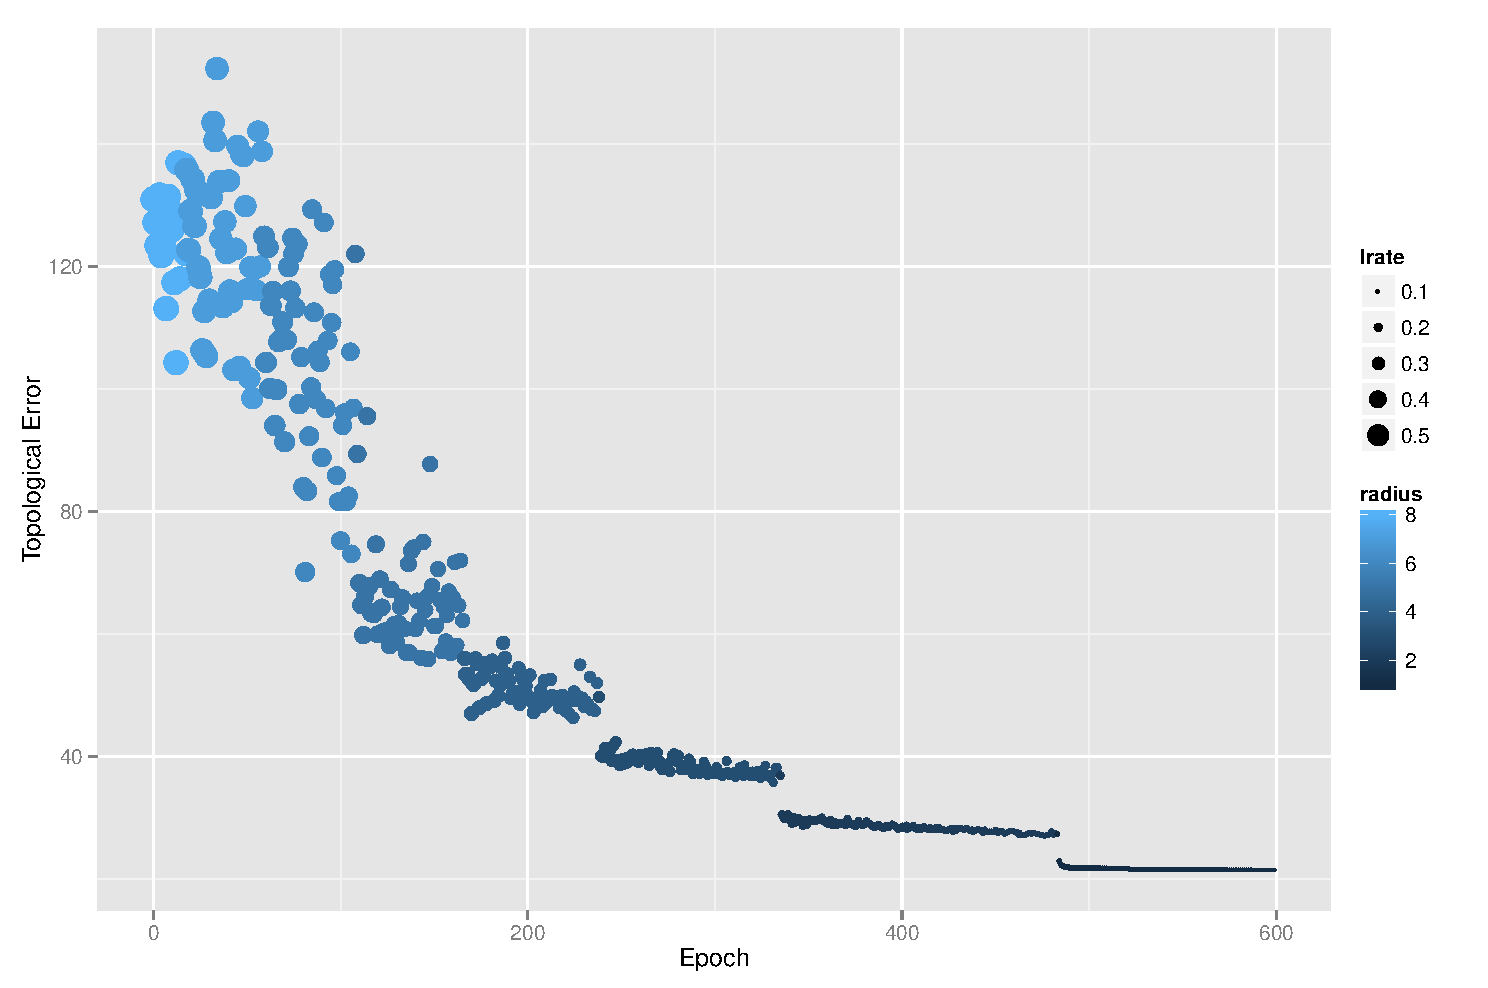
\includegraphics[scale=0.6]{./plots/som/topological_error.pdf}
  \label{fig:top_error}
  \caption{Changes in topological error throughout the SOM training, lrate stands for learning rate, and radius for radius applied to the winning neuron}
\end{figure}

\begin{figure}[h]
  \centerline{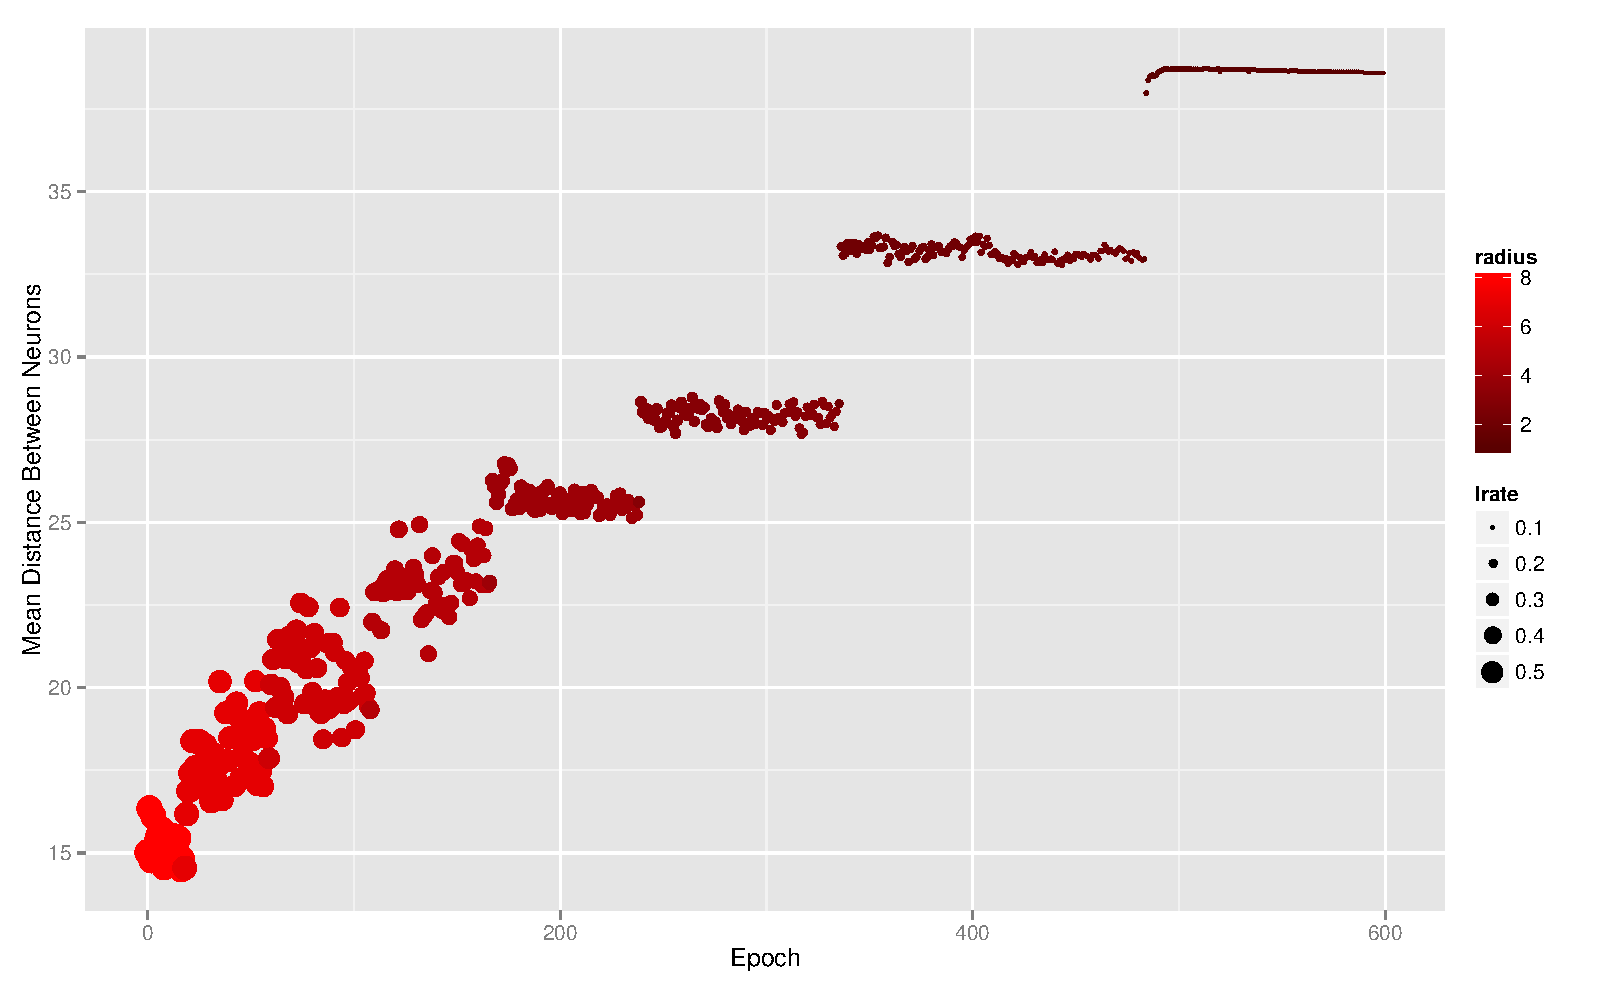
\includegraphics[scale=0.6]{./plots/som/average_distance.pdf}}
  \label{fig:avg_dist}
  \caption{Changes in the average distance between neurons, throughout the SOM training}
\end{figure}

\begin{figure}[htpb]
  \centering
  \subfigure[Output Space]{
\includegraphics[scale=1]{./images/som_training/1_som.pdf}\label{chp3:onesom}}
  \hspace*{0.5cm}
  \subfigure[U-Matrix]{
\includegraphics[scale=0.5]{./images/som_training/1_umatrix.pdf}\label{chp3:onematrix}}
  \hspace*{0.5cm}
  \subfigure[Q-Matrix]{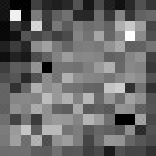
\includegraphics[scale=1]{./images/som_training/1_quantmatrix.pdf}\label{chp3:onetopmat}}
  \hspace*{0.5cm}
  \caption{ SOM state after first epoch of training. Its learning rate is at 0.598, and radius at 8.  }
  \label{fig:}
\end{figure}

\begin{figure}[htpb]
  \centering
  \subfigure[Output Space]{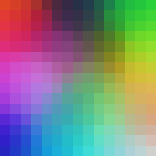
\includegraphics[scale=1]{./images/som_training/2_som.pdf}\label{chp3:onesom}}
  \hspace*{0.5cm}
  \subfigure[U-Matrix]{
\includegraphics[scale=0.5]{./images/som_training/2_umatrix.pdf}\label{chp3:onematrix}}
  \hspace*{0.5cm}
  \subfigure[Q-Matrix]{
\includegraphics[scale=1]{./images/som_training/2_quantmatrix.pdf}\label{chp3:onetopmat}}
  \hspace*{0.5cm}
  \caption{ SOM state after second epoch of training. Its learning rate is at 0.22, and radius at 3.  }
  \label{fig:}
\end{figure}

\begin{figure}[htpb]
  \centering
  \subfigure[Output Space]{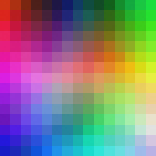
\includegraphics[scale=1]{./images/som_training/3_som.pdf}\label{chp3:onesom}}
  \hspace*{0.5cm}
  \subfigure[U-Matrix]{
\includegraphics[scale=0.5]{./images/som_training/3_umatrix.pdf}\label{chp3:onematrix}}
  \hspace*{0.5cm}
  \subfigure[Q-Matrix]{
\includegraphics[scale=1]{./images/som_training/3_quantmatrix.pdf}\label{chp3:onetopmat}}
  \hspace*{0.5cm}
  \caption{ SOM state after third epoch of training. Its learning rate is at 0.081, and radius at 1.  }
  \label{fig:}
\end{figure}

\begin{figure}[htpb]
  \centering
  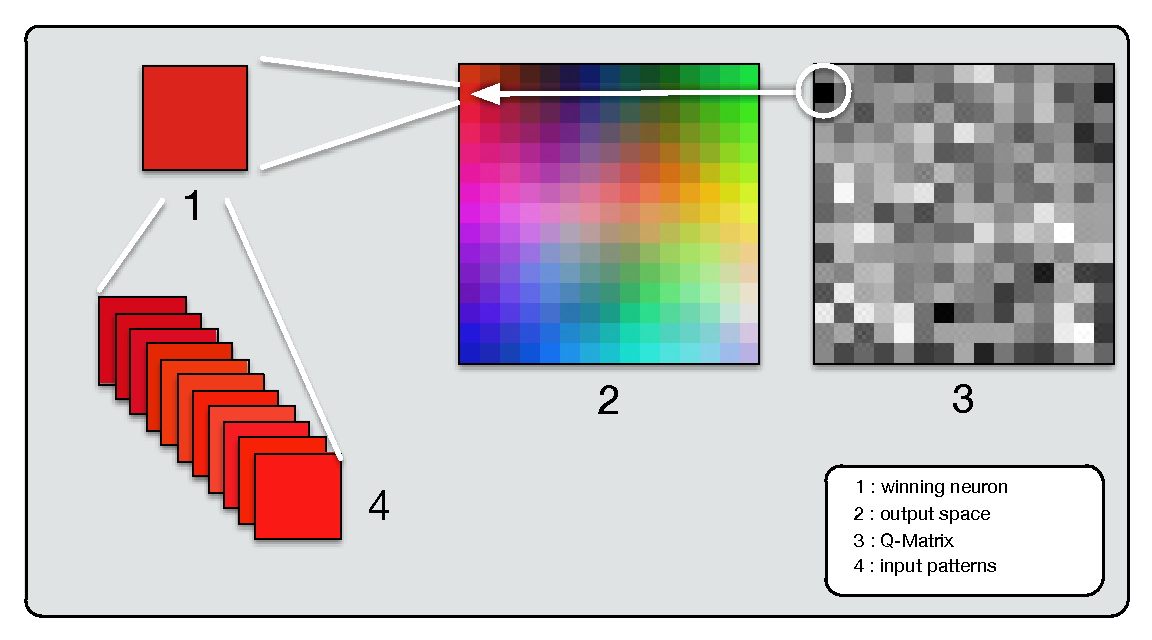
\includegraphics[width=0.8\linewidth]{./images/som_trainned.pdf}
  \caption{Input patterns associated with the neuron with maximum topological error --31. Even though the neuron has the biggest topological error of all neurons, it still has a good representation of the input patterns. The colors in this image are not figurative, and represent the entities at the end of trainning  }
  \label{fig:./images/som_trainned}
\end{figure}

\subsection{Benchmarking}
\label{sub:benchmarking}

 


\section{Conclusions}
{\color{red} Only these methods are not enough to cluster tweets }

% Ensure that the next chapter starts in a odd page
\cleardoublepage
 
%%%%%% REMOVED STUFF
%\subsection{Topology Preservation} 
%\label{sub:topology_preservation}
%The Self-Organizing Map performs a mapping from the n-dimensional input space into the two dimensional output space and where resides one the most fascinating characteristics, which is that the output map tries to preserve the topology from the input space. This grants the SOM algorithm a way to visualize high-dimensional data that other neural networks or clustering algorithms don't have. Even though this is true, sometimes during training it is not possible to preserve the topology of the network.
%Thus topology preservation can be measured through the Topographic error~\citet{Kiviluoto1996} which is the proportion of all data vectors for which first and second BMUs \footnote{unit that is closest to the winning neuron. BMU Best fitting unit } are not adjacent units.
%In this project the Topographic Error will be calculated for all SOM implementations and VSM usages in order to understand if the representation of the SOM output space is well defined.

 %\begin{itemize}
  %\item show UMatrixes and multiple steps map trainning of the SOM library trainnig
  %\item show metrics for the crawller, tweets per second, users persecond, size of the dump a long the time.
  %\item compare my som library with other som libraries: training velocity with diferent parameters, map after trainned.
  %\item Compare Homophilic-SOM results with non homophilic: UMatrixes, cluster results, Quantization error, jacknife. 
%\end{itemize}
%%\section{Evaluation Metrics} 
%%\label{sec:evaluation_metrics}
%Evaluation of the topic detection on Tweets will be made in two distinct ways. The first way will focus on  binary classification using the precision and recall metrics, and will be described in Subsection~\ref{sub:testing_for_precision_and_recall}. The second way will focus on statistically testing the SOM learning process and the computed trained network. This testing process will be described in Subsection~\ref{sub:cluster_quality_testing}. 

%\section{Testing for Precision and Recall} 
%\label{sec:testing_for_precision_and_recall}
%Precision and Recall are both ways to measure the rate of right guesses made by the trained SOM network, and are defined in the following way:
%\begin{itemize}
  %\item \textbf{Precision:} Fraction of retrieved instances that where relevant 
    %\begin{equation}
  precision = \frac{|{relevant\;documents}\cap{retrieved\;documents}|}{{retrieved\;documents}}
\end{equation} 

  %\item \textbf{Recall:} Fraction of relevant instances that where retrieved
    %\begin{equation}
  recall = \frac{|{relevant\;documents}\cap{retrieved\;documents}|}{{relevant\;documents}} 
\end{equation} 

%\end{itemize}
 
%In order to calculate Precision and Recall we need to have the \emph{relevant documents} and the \emph{retrieved documents}. The \emph{relevant documents} are rather hard to determine because they need to be categorized by humans, which is an expensive task.

\fancychapter{Conclusions and Future Work}
Draw your conclusions here and sell your work. Trasmit to the juri how hard it was to develop the presented work.

A future work section is usually here.

% Ensure that the next chapter starts in a odd page
\cleardoublepage
 


\pdfbookmark[0]{Bibliography}{bib}
\bibliographystyle{apalike}
\bibliography{bibliographies/library,bibliographies/sites}
\cleardoublepage   
\appendix
% %%%%%%%%%%%%%%%%%%%%%%%%%%%%%%%%%%%%%%%%%%%%%%%%%%%%%%%%%%%%%%%%%%%%%%
% First appendix
% %%%%%%%%%%%%%%%%%%%%%%%%%%%%%%%%%%%%%%%%%%%%%%%%%%%%%%%%%%%%%%%%%%%%%%
\fancychapter{Appendix A}
\label{ch:rsom_training}
\begin{figure}[htpb]
  \centering
  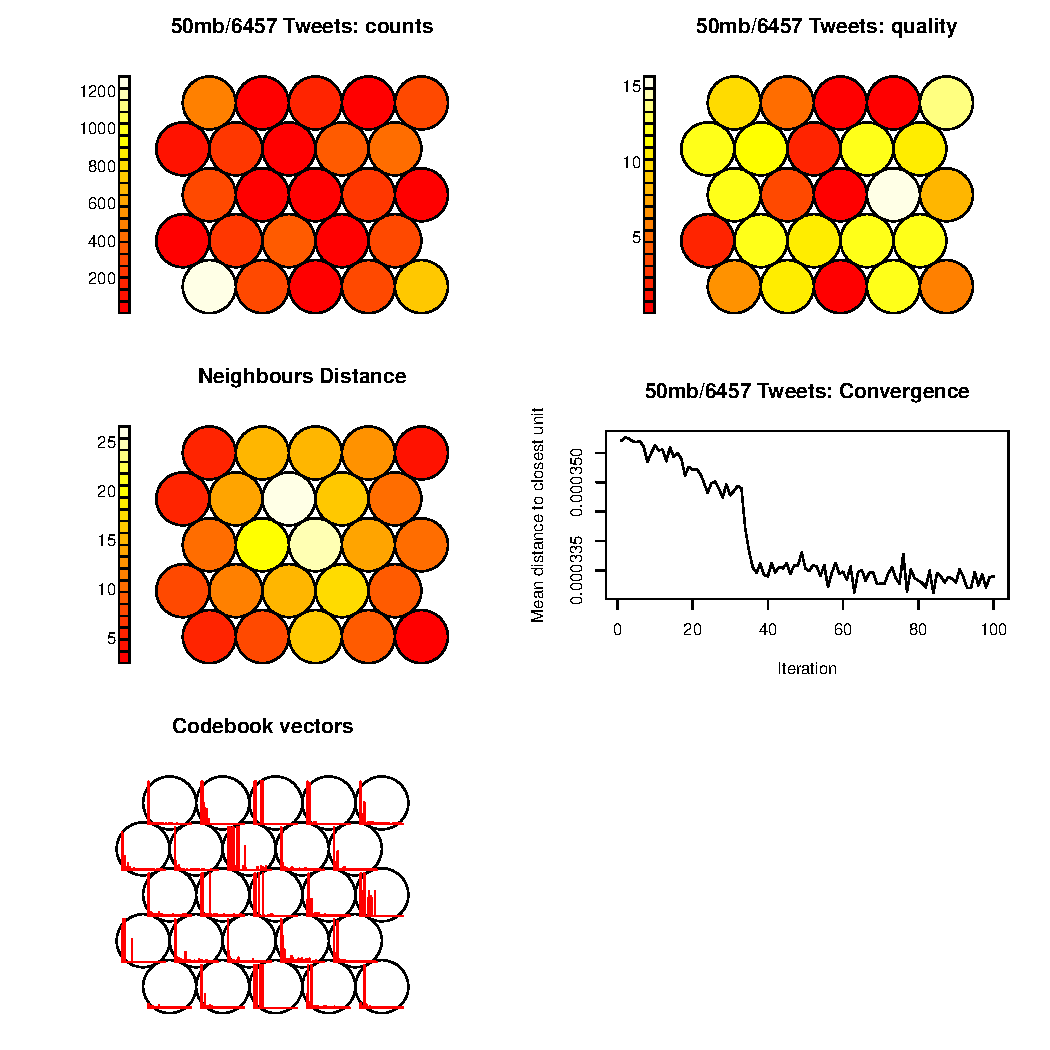
\includegraphics[width=0.8\linewidth]{./images/50mb_6457tweets_dataset.pdf}
  \caption{Training data for 6457 tweets. The counts map, shows us how many tweets are mapped to each cluster. Quality shows the mean distance of objects mapped to a unit to the codebook vector, the smaller the distance the better the representation. The neighborhood disance show the U-Matrix and finally the tweets convergence shows the distance from each node's wheights to the samples represented by that node }
  \label{fig:somr_images}
\end{figure}

\cleardoublepage

% %%%%%%%%%%%%%%%%%%%%%%%%%%%%%%%%%%%%%%%%%%%%%%%%%%%%%%%%%%%%%%%%%%%%%%
% Second appendix
% %%%%%%%%%%%%%%%%%%%%%%%%%%%%%%%%%%%%%%%%%%%%%%%%%%%%%%%%%%%%%%%%%%%%%%
%\fancychapter{Appendix A}
%\cleardoublepage  

\end{document}
